\chapter{Implementation}
\label{cha:implementation}

\epigraph{Ideas are easy, Implementation is hard.}{Guy Kawasaki}

Most of the implementation details and general decisions made for developing a
real-world functional project, based on the design architecture presented in chapter
\ref{cha:architecture}, are discussed in this chapter. It is organized in such a
way that it starts with the foundation and then progresses to the autoscaling of
worker nodes before moving on to example deployments of various applications in the
cluster. \\ %
The technology and programming languages utilized in the implementation are heterogeneous.
Nevertheless, according to a shared set of APIs and pre-defined structures, they
interact as a distinct and homogenous entity that maintains the entire cluster
in an active and healthy state. \\ %
Furthermore, several of the components and/or technologies discussed in this chapter
are interchangeable with other solutions. The latter is highly valuable for
organizations since it provides more configuration freedom and final control
over the cluster while continuously reflecting its ultimate goal. \\ %
The main implementation of the cluster and its related applications currently
supports the \texttt{Linux} platform (see section
\ref{subsec:architecture_components_node}) together with the architectures \texttt{amd64}\footnote{\url{https://wikipedia.org/wiki/X86-64}},
arm32\footnote{\url{https://wikipedia.org/wiki/ARM_architecture_family}} and \texttt{arm64}\footnote{\url{https://wikipedia.org/wiki/AArch64}}.

\section{Distributions}
\label{sec:implementation_distributions}

% TODO Reference introduction dependencies

Almost all software relies on the necessity for a stable and consistent
operating system (OS). \\ %
The OS, as specified in section \ref{subsec:architecture_components_node}, is
installed on every node in the cluster and must be based on the \texttt{Linux
Kernel}. The latter is a critical requirement because most of the technologies
employed in the implementation rely on Linux primitives and core functionality
to operate properly. To enforce resource management for pods and containers, for
example, all Kubernetes distributions require the \texttt{cgroup v2}\footnote{\url{https://www.kernel.org/doc/html/latest/admin-guide/cgroup-v2.html}}
kernel module\footnote{\url{https://kubernetes.io/docs/concepts/architecture/cgroups}}.
Furthermore, the Linux Kernel is an Open Source project to which everyone can
contribute and get access, representing one fundamental objective of the entire project.
\\ %
To represent the potential of the implementation architecture being compatible with
several Linux distributions, the section is titled Distributions rather than
Operating System. A Linux distribution, often known as a Linux distro, is an operating
system that is built from components developed by various open-source projects and
programmers. The Linux kernel (the operating system's core), the GNU shell utilities
(terminal interface and commands), the X server (for a graphical desktop), the desktop
environment, a package management system, an installer, and other services are
all included in each distribution. Many components are created independently and
released in source code format. Thousands of software packages, utilities, and
applications can be found in a single Linux distribution. Linux distributions combine
code from open-source projects into a single operating system that can be installed
and booted. Linux distributions are available for a wide range of specialized
use cases, including desktop computers, servers without a graphical interface, supercomputers,
mobile devices, and more\cite{linux_distro}. \\ %
To be completely compatible with the implementation architecture, a Linux distribution
must meet three major requirements. They are described in the following list:
\begin{enumerate}
  \item The Linux Kernel version must be compatible with the Kubernetes version.
    \newline
    Newer versions of K8s may require newer versions of the Linux Kernel to
    provide newer functions and/or improve overall security.

  \item All necessary packages, as explained and documented in the section
    \ref{subsec:implementation_distributions_packages}, must be installed and globally
    accessible in the system.
    \newline
    A check on all essential packages is performed before the execution of the
    installation program, as detailed in section \ref{sec:implementation_installer}.
    If even one package is missing from the system, the installation fails with an
    error message identifying the missing packages.

  \item An Init System that is supported and compatible, as defined in the
    section \ref{subsec:implementation_distributions_init_system}.
    \newline
    OpenRC and Systemd are supported by the implementation. They are currently
    the two most used init systems, and the majority of available distributions are
    based on one of them.
\end{enumerate}
Finally, two custom Linux distributions are already configured, built, and
packaged as ISO files, as shown in section \ref{subsec:implementation_distributions_iso_image}.
They are based on a simple command line with no graphical interface and contain
only what is required to start a node. This is done to simplify the overall setup
by eliminating unnecessary software and technologies, addressing any
incompatibilities, and increasing the cluster's implementation and testing efficiency.
Both are derived from pre-existing Linux distributions that are known to be
stable, easy to configure, and lightweight, requiring just the bare minimum of resources
to operate. Furthermore, they are built on separate init systems, requiring the
overall implementation to be compatible with and tested with both.

\subsection{Packages}
\label{subsec:implementation_distributions_packages}

The packages used in the implementation that must be available in a Linux distribution
are specified in this section. A package is a collection of files that have been
bundled together and may be installed and uninstalled as a group\cite{package_manager}.
\\ %
All packages may be installed automatically using the package manager of the respective
Linux distribution. A package manager's job is to provide an interface that
assists the user in managing the collection of packages installed on the system.
A package manager maintains track of what software is installed on the system and
makes it simple to install new software, update software to newer versions, or delete
previously installed software. A package is usually a single piece of software. However,
it is typical for applications to be made up of numerous dependent packages. For
example, the \texttt{jq} package includes not just the \texttt{jq} command-line
JSON processor, but also the \texttt{oniguruma}\footnote{\url{https://github.com/kkos/oniguruma}}
package, a regular expressions library. Furthermore, various optional add-on packages
including extra data and documentation are available\cite{package_manager}. \\ %
All packages are already included by default in the two custom Linux
distributions. As a result, there is no need for any changes or the installation
of extra packages. \\ %
Each package in table \ref{tbl:packages} contains a brief description extracted
from its official documentation, as well as some notes on why it was utilized.
Furthermore, the required column indicates with symbols if the package is required
(\textcolor{bulmaGreen}{\faicon{check}}), optional (\textcolor{bulmaBlue}{\faicon{question}}),
or not required (\textcolor{bulmaRed}{\faicon{times}}). It should be noted that the
name of some packages may differ based on the package manager employed by the Linux
distribution.

\begin{xltabular}
  {\textwidth} { >{\ttfamily}l | c | X | X }

  \multicolumn{1}{ c |}{\large{\textbf{Name}}} &
  \multicolumn{1}{ c |}{\large{\textbf{Required}}} &
  \multicolumn{1}{ c |}{\large{\textbf{Description}}} &
  \multicolumn{1}{ c }{\large{\textbf{Notes}}} \\ \hhline{====}

  bc & \textcolor{bulmaGreen}{\faicon{check}} & \texttt{bc}, also known as basic
  calculator, is a language that allows for arbitrary precision numbers with
  interactive statement execution\cite{bc}. & The Linux terminal does not
  support complicated math operations or number comparisons. As a result, the
  \texttt{bc} program is used throughout the installation procedure to guarantee
  that computed data, such as the node's mean power consumption and Simple
  Standard Deviation\footnote{\url{https://wikipedia.org/wiki/Standard_deviation}},
  is neither less than nor more than a threshold value. \\ \hline

  coreutils & \textcolor{bulmaGreen}{\faicon{check}} & The GNU Core Utilities
  are the GNU\footnote{\url{https://www.gnu.org}} operating system's essential
  file, shell, and text manipulation utilities. These are the core utilities that
  are required to be included in any operating system\cite{coreutils}. & By default,
  minimal Linux distributions only include a portion of the massive list of
  utilities provided in the standard \texttt{coreutils} package. As a result, several
  of the applications utilized in the implementation are missing. Therefore, the
  whole \texttt{coreutils} package is required. \\ \hline

  docker & \textcolor{bulmaBlue}{\faicon{question}} & Docker Engine is a container
  engine that allows creating, managing, and operating OCI\footnote{\url{https://opencontainers.org}}
  (Open Container Initiative) Containers on a Linux system\cite{docker}. & During
  the cluster initialization procedure, \texttt{docker} is widely utilized to tag\footnote{\url{https://docs.docker.com/engine/reference/commandline/tag}}
  and push\footnote{\url{https://docs.docker.com/engine/reference/commandline/push}}
  various container images corresponding to specific implementation dependencies
  (see section \ref{sec:implementation_dependencies}) to the private registry.
  It should be noted that \texttt{docker} is not the only tool for working with OCI
  containers, hence the optional symbol, but it is the most popular with well-known
  and simple CLI commands. As an example, \texttt{podman}\footnote{\url{https://podman.io}}
  is a Docker-compatible command line front end that can simply alias the Docker
  CLI (\texttt{alias docker=podman}), requiring no modifications to the
  implementation code\cite{podman}. \\ \hline

  ethtool & \textcolor{bulmaGreen}{\faicon{check}} & \texttt{ethtool} is a standard
  Linux software for managing network drivers and hardware by modifying Network Interface
  Controller (NIC) settings\cite{ethtool}. & If the node's NIC interface supports
  Wake-on-Lan (WoL), \texttt{ethtool} is used to activate it.
  \newline
  It's worth noting that the NIC interface may reset to factory settings
  following a reboot. As a result, \texttt{ethtool} is always run before the NIC
  interface is activated. \\ \hline

  grep & \textcolor{bulmaGreen}{\faicon{check}} & \texttt{grep} prints lines from
  input files or standard input that match one or more patterns\cite{grep}. & \texttt{grep}
  is an essential utility in all Linux systems. It is widely utilized in all scripts
  for matching predetermined patterns and executing arbitrary actions based on the
  latter's results. \\ \hline

  inotify-tools & \textcolor{bulmaGreen}{\faicon{check}} & Monitor one or more
  files or directories for a predefined set of events, such as open, close, move/rename,
  delete or create. Under the hood, to be more efficient, it makes use of Linux's
  \texttt{inotify}\footnote{\url{https://docs.kernel.org/filesystems/inotify.html}}
  interface\cite{inotify_tools}. & Obtaining access information to the
  underlying Kubernetes cluster is required during the cluster initialization
  phase. This information is only available in an automatically generated configuration
  file saved in a specific and well-known directory. As a result, before proceeding
  to the next phase, the installation script uses the \texttt{inotifywait} program
  to wait for the file to be created. \\ \hline

  iproute2 & \textcolor{bulmaGreen}{\faicon{check}} & \texttt{iproute2} is a collection
  of utilities for managing TCP/IP\footnote{\url{https://wikipedia.org/wiki/Internet_protocol_suite}}
  networking and traffic control in Linux\cite{iproute2}.
  \newline
  The most essential tools are \texttt{ip} and \texttt{tc}. IPv4 and IPv6
  configuration is handled by \texttt{ip}, whereas \texttt{tc} stands for traffic
  control. & During the installation phase, the command \texttt{ip} is used to
  gather information about physical network interfaces that are not \texttt{loopback}\footnote{\url{https://wikipedia.org/wiki/Loopback}},
  such as name and MAC address. \\ \hline

  jq & \textcolor{bulmaGreen}{\faicon{check}} & \texttt{jq} is a lightweight and
  flexible command-line JSON\footnote{\url{https://www.json.org}} processor\cite{jq}.
  & To manipulate JSON data, all scripts make extensive use of \texttt{jq}. \\ \hline

  ncurses & \textcolor{bulmaRed}{\faicon{times}} & The \texttt{ncurses} (new curses)
  library is a free software emulation of curses in System V\footnote{\url{https://wikipedia.org/wiki/UNIX_System_V}}.
  It supports pads, color, multiple highlights, forms characters, and function-key
  mapping, as well as all of the other SVr4-curses improvements over BSD curses\cite{ncurses}.
  & The \texttt{ncurses} package includes the \texttt{tput} software, which is a
  utility for retrieving terminal capabilities in shell scripts.
  \newline
  When the spinner process is spawned in a script, \texttt{tput} is used to
  update its symbols at regular intervals, replacing the old one with the new one
  and updating the cursor position. Because a spinner is only a decorative
  element, the package is not required and can be omitted. \\ \hline

  nodejs & \textcolor{bulmaBlue}{\faicon{question}} & Node.js is an open-source,
  cross-platform JavaScript\footnote{\url{https://developer.mozilla.org/docs/Web/JavaScript}}
  runtime environment\cite{nodejs}. & This package is optional since the Server component,
  see section \ref{subsec:architecture_components_server}, may be bundled as a single
  binary or in a container, removing the need for the \texttt{nodejs} package to
  be installed. Because the present implementation does not provide any of the
  aforementioned alternatives, \texttt{nodejs} is included in both of the two
  custom Linux distributions. \\ \hline

  npm & \textcolor{bulmaBlue}{\faicon{question}} & The package manager for the Node.js
  JavaScript platform. It installs modules so that Node.js can locate them and
  intelligently resolves dependency conflicts. It is highly adaptable to serve a
  wide range of use cases. It is often used to publish, find, install, and build
  node applications\cite{npm}. & This package is optional since the Server component
  may be bundled as a single binary or in a container, removing the need for the
  \texttt{npm} package to be installed. Because the present implementation does
  not provide any of the aforementioned alternatives, \texttt{npm} is included
  in both of the two custom Linux distributions. \\ \hline

  openssh & \textcolor{bulmaGreen}{\faicon{check}} & The OpenSSH software suite includes
  tools for managing secure tunneling capabilities, various authentication
  methods, and advanced configuration options.
  \newline
  OpenSSH is the most popular remote login tool for the SSH protocol\footnote{\url{https://wikipedia.org/wiki/Secure_Shell}}.
  It encrypts all traffic to prevent eavesdropping, connection hijacking, and other
  types of attacks\cite{openssh}. & OpenSSH is critical in the cluster for protecting
  remote operations, key management, and other tasks. All operations are
  inherently unsafe without its software and can pose serious security issues, especially
  if the cluster is accessible from external networks. \\ \hline

  postgresql & \textcolor{bulmaBlue}{\faicon{question}} & \texttt{PostgreSQL} is
  a powerful, open-source object-relational database system with a high
  reputation for reliability, feature robustness, and performance\cite{postgresql}.
  & \texttt{PostgreSQL} is the database implementation used for the Database component
  (see section \ref{subsec:architecture_components_database}).
  \newline
  This package is optional since the database may be implemented outside of the
  cluster using other solutions. It is up to the organization in charge of the cluster
  to decide whether or not the database package should be included in the Linux distribution.
  \\ \hline

  procps-ng & \textcolor{bulmaRed}{\faicon{times}} & \texttt{procps} is a collection
  of command-line and full-screen programs that offer information from the \texttt{/proc}\footnote{\url{https://docs.kernel.org/filesystems/proc.html}}
  pseudo-filesystem. \texttt{procps} programs often concentrate on the structures
  that describe the processes operating on the system\cite{procps_ng}. & The \texttt{procps-ng}
  package includes the \texttt{ps} software, which displays information about
  the system's active processes.
  \newline
  When the spinner process is spawned in a script, \texttt{ps} is used to obtain
  the PID\footnote{\url{https://wikipedia.org/wiki/Process_identifier}} of the parent
  process. Because a spinner is only a decorative element, the package is not required
  and can be omitted. \\ \hline

  sed & \textcolor{bulmaGreen}{\faicon{check}} & \texttt{sed} is a stream editor.
  A stream editor is used on an input stream (file or standard input) to perform
  simple filtering and text transformations. While comparable to an editor that allows
  scripted edits, \texttt{sed} operates by making only one pass through the input(s)
  and is thus more efficient\cite{sed}. & \texttt{sed} is an essential utility in
  all Linux systems. It is widely utilized in all scripts for extracting well-defined
  portions and/or filtering data from its input(s). \\ \hline

  sudo & \textcolor{bulmaGreen}{\faicon{check}} & \texttt{sudo} (su\footnote{\url{https://wikipedia.org/wiki/Su_(Unix)}}
  "do") enables a system administrator to delegate authority to allow specific users
  (or groups of users) to run certain (or all) commands as root or another user while
  providing an audit record of the commands and their arguments. \texttt{sudo} works
  on a per-command basis; it is not a shell replacement\cite{sudo}. & The
  installation phase involves actions that need administrative authorization. Before
  performing any processing, the script checks to see whether the current user
  already has root\footnote{\url{https://wikipedia.org/wiki/Superuser}}
  privileges; if not, it requests them with \texttt{sudo}. \\ \hline

  sysbench & \textcolor{bulmaGreen}{\faicon{check}} & \texttt{sysbench} is a multithreaded
  scriptable benchmark tool for measuring CPU, memory, file I/O, mutex
  performance, and database performance\cite{sysbench}. & During the installation
  phase, \texttt{sysbench} is extensively used to analyze a cluster node's performance
  and, in conjunction with other tools, its power consumption. \\ \hline

  tar & \textcolor{bulmaGreen}{\faicon{check}} & \texttt{tar} is an archiving application
  that can store and manipulate numerous files in a single file (an archive).
  The archive can be either a standard file or a device, which can be placed on a
  local or remote system\cite{tar}. & \texttt{tar} is primarily used in
  production during the installation process to extract and manipulate various
  archive files.
  \newline
  \texttt{tar} is used in development to create the bundle archive for
  distribution, which contains all files and applications. \\ \hline

  tzdata & \textcolor{bulmaGreen}{\faicon{check}} & The Time Zone Database is a
  collection of code and data that represents the history of local time for
  several representative locations all over the world. It is updated regularly to
  reflect changes in time zone boundaries, UTC offsets, and daylight-saving laws
  enacted by legislative entities\cite{tzdata}. & To avoid date and time inconsistencies,
  all nodes in the cluster must be configured to the same timezone. By default,
  all nodes are configured to the Etc/UTC timezone. \\ \hline

  util-linux & \textcolor{bulmaGreen}{\faicon{check}} & \texttt{util-linux} is a
  random collection of Linux utilities\cite{util_linux}. & The installation
  script makes use of two \texttt{util-linux} utility programs: \texttt{lscpu} to
  display information about the CPU architecture and \texttt{lsblk} to list
  block devices. \\ \hline

  yq & \textcolor{bulmaGreen}{\faicon{check}} & \texttt{yq} is a portable and
  lightweight command-line YAML\footnote{\url{https://yaml.org}}, JSON, and XML\footnote{\url{https://www.w3.org/XML}}
  processor.
  \newline
  \texttt{yq} has a syntax similar to \texttt{jq}. It does not cover all that
  \texttt{jq} supports, but it does support the majority of the most common
  operations and functions\cite{yq}. & To manipulate YAML data, all scripts make
  extensive use of \texttt{yq}.
  \newline
  \texttt{yq} is primarily used to read and save YAML files. However, because of
  its more advanced functions and solutions, \texttt{jq} is used for the
  majority of complex data processing, at the expense of \texttt{yq}. As a result,
  YAML structures are first transformed to/from JSON, then processed with \texttt{jq},
  and then converted back to/from YAML. The double conversion should be
  eliminated and/or simplified in future implementations. \\ \hline

  \caption{Packages list}
  \label{tbl:packages}
\end{xltabular}

\subsection{Init System}
\label{subsec:implementation_distributions_init_system}

The Init System, short for Initialization System, is the first process that runs
when a Unix-based computer operating system is bootstrapped. Init is a daemon
process that is normally given Process IDentifier 1 (PID 1) and runs until the
system is shut down. It is the direct or indirect ancestor of all other processes
and adopts all orphaned processes automatically. The kernel starts Init during
the boot process; if the kernel is unable to start it, a kernel panic occurs\cite{init_system}.
\\ %
The Init System is logically positioned above the Kernel and is an essential component
of every modern system. It frequently integrates sophisticated features over
simple ones and is very customizable. Furthermore, it offers active control and
monitoring over the running processes, keeping the entire system healthy and active.
The latter is critical because it enables automated and continuous monitoring of
cluster implementation architecture-related processes operating in the node
without the need for a custom solution. For example, if a K8s instance executing
in a worker node crashes (i.e. exits with a code different than 0), the Init
System detects it and restarts the process automatically, making the node active
and able to receive workload again. \\ %
When the node is bootstrapped, the Init System is set to start all cluster-related
processes (i.e., K8s instance and Metric Server) and run a script that sends a
message to the server component notifying it that the node is active and ready. Before
the node is shut down, it automatically terminates all cluster-related processes
and sends a message to the server component informing that the node is shutting
down and will be inactive. As previously stated, the cluster performs these two
operations automatically: bootstrap for upscaling and shutdown for downscaling.
However, there are scenarios in which a node is manually bootstrapped and/or shut
down by human action without involving the server component directly. Despite
the possibility of the latter, the overall cluster state remains consistent, and
all node statuses are correctly updated, thanks to the Init System and its monitoring
and configuration capabilities. \\ %
The implementation currently supports two init systems: OpenRC (described in section
\ref{subsec:implementation_distributions_init_system_openrc}) and Systemd (described
in section \ref{subsec:implementation_distributions_init_system_systemd}). They are
the two most popular and widely used Init Systems, and the vast majority of
Linux distributions support one or both of them. Their capabilities are nearly identical.
However, configuration files and available application(s) that interact with the
bare-metal Init System API, are different, necessitating double effort to
achieve the same objective. \\ %
It should be noted that if the Init System daemon process crashes due to an
error, the entire system crashes and becomes inactive, necessitating a manual
restart. Even though the likelihood of the latter is extremely low, it is never
zero. As a result, as stated in section
\ref{subsec:architecture_components_server}, a heartbeat mechanism has been established
in the cluster to constantly monitor and identify the status and availability of
all active nodes. If there are no configuration or networking issues and a node's
heartbeat is not received within the predefined interval, it indicates that the heartbeat
daemon executing in the node has crashed and has not yet been restarted, or that
the entire node has crashed and is not automatically recoverable. \\ %
In each of the following sections, where an Init System distribution is described,
an example of the related service configuration file is presented to illustrate
its differences. A service configuration file contains information about a process
that the Init System controls and monitors. The application used as a reference
in this example is K3s, a lightweight Kubernetes distribution explained in further
detail in section \ref{subsec:implementation_dependencies_k3s}. Before starting,
it must clear any temporary files in the \texttt{tmp} directory and load
environment variables from two distinct directories. Furthermore, anytime the
application process crashes, the Init System must restart it within 5 seconds after
detection. Even though each Init System has a unique service configuration file,
the result is nearly identical. The list below highlights some of the most
significant configuration requirements. To aid comprehension, the identification
number for each requirement is also provided in the Init System's service
configuration file.
\begin{enumerate}[label=\protect\circled{\arabic{*}}]
  \item General information about the service.
    \newline
    Useful for users and/or administrators.

  \item Services on which the service is dependent.
    \newline
    The listed services must be activated before the current service may start.

  \item Remove any temporary files that begin with the name \texttt{k3s} and are
    placed in the temporary (\texttt{tmp}) directory before launching the application.

  \item Type of service. Different types correspond to various service behaviors
    as well as how the application is monitored and regulated.
    \newline
    In this case, monitor the application process and restart it if there is a
    crash or an anomaly.

  \item Absolute path to the application's binary file.

  \item Application arguments.

  \item Waiting time in seconds before restarting the crashed application.

  \item The maximum number of restarts permitted. When the threshold is met, the
    program is no longer restarted.
    \newline
    A value of 0 indicates that no threshold exists and that the application has
    no restart limit.

  \item Load \texttt{/etc/environment} and \texttt{/etc/rancher/k3s/k3s.env} environment
    variables files before starting the application.
\end{enumerate}

\subsubsection{OpenRC}
\label{subsec:implementation_distributions_init_system_openrc}

\begin{wrapfigure}
  {r}{.25\textwidth} %
  \centering
  \def\stackalignment{r}\stackunder{ 
\includegraphics[width=\linewidth]{images/logos/gentoo.png} } %
  {\scriptsize \parbox[t]{\linewidth}{ Source: \url{https://www.gentoo.org/inside-gentoo/artwork/gentoo-logo.html}} }
  \caption{Gentoo Linux logo}
\end{wrapfigure}

OpenRC is a dependency-based init system for Unix-like systems that maintain
compatibility with the system's init system, which is generally found in \texttt{/sbin/init}.
\\ %
At boot, OpenRC starts the appropriate system services in the right sequence, manages
them while the system is running, and stops them at shutdown. It can manage installed
daemons, optionally monitor the processes it launches, and start processes in parallel
when possible to reduce boot time. \\ %
OpenRC was developed for Gentoo\footnote{\url{https://www.gentoo.org}}, but it
may be used in other Linux distributions and BSD\footnote{\url{https://www.bsd.org}}
systems as well\cite{openrc}. \\ %
Listing \ref{lst:openrc} illustrates the example of the OpenRC service configuration
file for K3s saved in \texttt{/etc/init.d/k3s}. Manual control of the service is
possible using the \texttt{rc-service} command, which locates and runs the
OpenRC service with the specified arguments: \texttt{rc-service k3s <CMD> [...]}.
\texttt{<CMD>} can be substituted by \texttt{start} to start the service,
\texttt{stop} to stop the service, \texttt{restart} to restart the service, and
\texttt{status} to acquire the service status. Furthermore, with the command \texttt{rc-update
add k3s default}, the service may be set to start automatically when the system boots
up. The latter examples are merely a very small subset of all the available
commands/capabilities that OpenRC is capable of.

\begin{lstlisting}[language=shell, escapeinside={(*@}{@*)}, morekeywords={[2]{depend, start_pre, want, after, sourcex}}, morekeywords={[4]{name, description, supervisor, command, command_args, output_log, error_log, pidfile, respawn_delay, respawn_max}}, xleftmargin=\parindent, label={lst:openrc}, caption=\texttt{OpenRC} service configuration file for K3s]
  #!/sbin/openrc-run

  name="k3s"                                                                                      (*@ \circled{\texttt{\tiny{1}}} @*)
  description="Lightweight Kubernetes"                                                            (*@ \circled{\texttt{\tiny{1}}} @*)

  depend() {
    want cgroups                                                                                  (*@ \circled{\texttt{\tiny{2}}} @*)
    after network-online                                                                          (*@ \circled{\texttt{\tiny{2}}} @*)
  }

  start_pre() {
    rm -f "/tmp/k3s.*"                                                                            (*@ \circled{\texttt{\tiny{3}}} @*)
  }

  supervisor="supervise-daemon"                                                                   (*@ \circled{\texttt{\tiny{4}}} @*)
  command="/usr/local/bin/k3s"                                                                    (*@ \circled{\texttt{\tiny{5}}} @*)
  command_args="server"                                                                           (*@ \circled{\texttt{\tiny{6}}} @*)
  output_log="/var/log/k3s.log"
  error_log="/var/log/k3s.log"
  pidfile="/var/run/k3s.pid"
  respawn_delay=5                                                                                 (*@ \circled{\texttt{\tiny{7}}} @*)
  respawn_max=0                                                                                   (*@ \circled{\texttt{\tiny{8}}} @*)

  set -o allexport
  if [ -f "/etc/environment" ]; then sourcex "/etc/environment"; fi                               (*@ \circled{\texttt{\tiny{9}}} @*)
  if [ -f "/etc/rancher/k3s/k3s.env" ]; then sourcex "/etc/rancher/k3s/k3s.env"; fi               (*@ \circled{\texttt{\tiny{9}}} @*)
  set +o allexport
\end{lstlisting}

\subsubsection{systemd}
\label{subsec:implementation_distributions_init_system_systemd}

\begin{wrapfigure}
  {r}{.25\textwidth} %
  \centering
  \def\stackalignment{r}\stackunder{ 
\includegraphics[width=\linewidth]{images/logos/systemd.png} } %
  {\scriptsize \parbox[t]{\linewidth}{ Source: \url{https://brand.systemd.io}} }
  \caption{systemd logo}
\end{wrapfigure}

systemd is a collection of building blocks for a Linux system. It provides a
system and service manager that runs as PID 1 and starts the rest of the system.
\\ %
systemd supports aggressive parallelization, on-demand daemon startup, process
tracking through Linux control groups, mount and automount point management, and
a complex transactional dependency-based service control logic. \\ %
Other components include a logging daemon, tools to handle basic system configuration
such as the hostname, date, and locale, a list of logged-in users and running
containers and virtual machines, system accounts, runtime directories and
settings, and daemons to manage simple network configuration, network time
synchronization, log forwarding, and name resolution\cite{systemd}. \\ %
Listing \ref{lst:systemd} illustrates the example of the systemd service configuration
file for K3s saved in \texttt{/etc/systemd/system/k3s.service}. The \texttt{systemctl}
command, which manages the systemd system and the service manager, may be used to
manually control the service: \texttt{systemd <CMD> k3s [...]}. \texttt{<CMD>} can
be replaced with \texttt{start} to start the service, \texttt{stop} to stop it, \texttt{restart}
to restart it, and \texttt{status} to obtain the service status. Furthermore,
the service may be enabled to start automatically when the system boots up by
using the commands \texttt{systemctl enable k3s} followed by \texttt{systemctl daemon-reload}
to reload the systemd management configuration. The latter examples are only a small
portion of all the commands and capabilities provided by systemd.

\begin{lstlisting}[language=ini, escapeinside={(*@}{@*)}, morekeywords={Description, Documentation, Wants, After, StartLimitBurst, WantedBy, Type, ExecStartPre, ExecStart, EnvironmentFile, KillMode, Delegate, TimeoutStartSec, Restart, RestartSec}, xleftmargin=\parindent, label={lst:systemd}, caption=\texttt{systemd} service configuration file for K3s]
  [Unit]
  Description=Lightweight Kubernetes                                                              (*@ \circled{\texttt{\tiny{1}}} @*)
  Documentation=https://k3s.io                                                                    (*@ \circled{\texttt{\tiny{1}}} @*)
  Wants=network-online.target                                                                     (*@ \circled{\texttt{\tiny{2}}} @*)
  After=network-online.target                                                                     (*@ \circled{\texttt{\tiny{2}}} @*)
  StartLimitBurst=0                                                                               (*@ \circled{\texttt{\tiny{8}}} @*)

  [Install]
  WantedBy=multi-user.target

  [Service]
  Type=notify                                                                                     (*@ \circled{\texttt{\tiny{4}}} @*)
  ExecStartPre=/usr/bin/env sh -c 'rm -f "/tmp/k3s.*"'                                            (*@ \circled{\texttt{\tiny{3}}} @*)
  ExecStart=/usr/local/bin/k3s server                                                         (*@ \hspace*{1.375pt} \circled{\texttt{\tiny{5}}} \circled{\texttt{\tiny{6}}} @*)
  EnvironmentFile=-/etc/environment                                                               (*@ \circled{\texttt{\tiny{9}}} @*)
  EnvironmentFile=-/etc/rancher/k3s/k3s.env                                                       (*@ \circled{\texttt{\tiny{9}}} @*)
  KillMode=process
  Delegate=yes
  TimeoutStartSec=0
  Restart=always                                                                                  (*@ \circled{\texttt{\tiny{4}}} @*)
  RestartSec=5s                                                                                   (*@ \circled{\texttt{\tiny{7}}} @*)
\end{lstlisting}

\subsection{ISO Image}
\label{subsec:implementation_distributions_iso_image}

This section briefly describes the two original Linux distributions, Alpine
Linux and Arch Linux, which served as the foundation for the two custom Linux distributions.
They were both utilized and tested together in the implementation cluster. Furthermore,
it is shown how the two custom ISO image files are customized and generated by
the use of a simple script. \\ %
Each customized Linux distribution comes in the form of a single ISO image file.
A disk image that contains everything that would be written on an optical disc,
including the optical disc file system, is known as an optical disc image (or
ISO image). ISO images are intended to include the binary image of an optical
media file system, as well as the data in its binary files, replicated exactly
as they were saved on the disc. The data included within the ISO image will be structured
in accordance with the file system used on the optical disc from which it was produced\cite{iso}.
\\ %
The ISO image can be burned into physical media such as a CD, or a USB flash drive
or can be mounted as an ISO file. The latter shows the high level of flexibility
and overall compatibility that an ISO file has. Moreover, it is extremely
portable since it is intrinsically only a single file making it the perfect
format for a release bundle and very useful in an Air-Gap environment. \\ %
After an ISO image of a Linux distribution has been burned to media, it can be easily
installed on multiple systems by attaching the media to the system and selecting
it as the default boot. It starts a live (volatile) OS that is not currently
installed on the primary disk. The live Linux distribution may then be installed
directly into the primary disk, making it permanently available on the system
without the need for removable media. The latter step may be performed manually,
but it is more complex than it appears since it necessitates an understanding of
disk formatting, partitioning, as well as other topics. Fortunately, most Linux
distributions, including the two custom ones, have simple tools that automate
the installation procedure by asking only a few simple questions to the user/administrator.

\subsubsection{Alpine Linux}
\label{subsubsec:implementation_distributions_iso_alpine_linux}

\begin{wrapfigure}
  {r}{.25\textwidth} %
  \centering
  \def\stackalignment{r}\stackunder{ 
\includegraphics[width=\linewidth]{images/logos/alpine.png} } %
  {\scriptsize \parbox[t]{\linewidth}{ Source: \url{https://alpinelinux.org}} }
  \caption{Alpine Linux logo}
\end{wrapfigure}

Alpine Linux\footnote{\url{https://www.alpinelinux.org}} is a lightweight, security-focused,
and resource-efficient distribution. In recent years, has grown in popularity as
the foundation for the majority of Docker images. It is based on musl\footnote{\url{https://musl.libc.org}}
(an implementation of the C standard library, an alternative to glibc\footnote{\url{https://www.gnu.org/software/libc}}),
BusyBox\footnote{\url{https://busybox.net}} (a single, small executable that combines
tiny versions of many common UNIX utilities), a custom package manager called APK\footnote{\url{https://wiki.alpinelinux.org/wiki/Alpine_Package_Keeper}}
and the OpenRC Init System (see section
\ref{subsec:implementation_distributions_init_system_openrc})\cite{alpine_linux}.
\\ %
Alpine Linux is the preferred reCluster distribution since it has been widely
used and tested throughout the development process.

The official documentation\footnote{\url{https://wiki.alpinelinux.org/wiki/How_to_make_a_custom_ISO_image_with_mkimage}}
provides a brief guideline on how to build a custom Alpine Linux ISO image. Unfortunately,
it is not exhaustive, and it assumes a lot of information and configurations. A
simpler, easy-to-use, and portable solution is required for cluster
implementation. This resulted in the creation of a POSIX script that handles all
of the burdens, as explained below. \\ %
Building a custom Alpine Linux ISO image involves three prerequisites: an Alpine
Linux system, specific tools/packages to configure and build the image, and a general
configuration with a special administrator user and the generation of signing keys.
These requirements remain constant over time and can be regarded as essentially
static. Furthermore, having a physical Alpine Linux system dedicated just to
generating custom images is a waste of resources. As a result, a custom
Dockerfile based on Alpine Linux has been created to allow building the image in
different environments without the need for a physical machine and with all of
the previous requirements already fulfilled\footnote{\url{https://github.com/carlocorradini/reCluster/blob/main/distributions/alpine/Dockerfile}}.
A Dockerfile is a text document that contains all of the commands needed to compile
a container image\cite{dockerfile}. \\ %
The ISO image is customized using the \texttt{mkimg.recluster.sh}\footnote{\url{https://github.com/carlocorradini/reCluster/blob/main/distributions/alpine/mkimg.recluster.sh}}
file, which defines and integrates a custom recluster profile, based on the basic
Alpine Linux profile. This file, whose content is shown in listing \ref{lst:alpine},
is not included in the Dockerfile because it is considered dynamic, in the sense
that it could be updated and customized over time to meet potential new cluster specifications.
\\ %
Finally, to create the ISO image, the container image must be launched in detached
mode, a local volume mounted to the container, the \texttt{mkimg.recluster.sh}
file loaded, and the official \texttt{mkimage.sh} script executed with extra
configuration parameters. When performed manually, the latter tasks are
extremely difficult and prone to human error. As a result, all operations have
been included in a POSIX script, simply named \texttt{build.sh}\footnote{\url{https://github.com/carlocorradini/reCluster/blob/main/distributions/alpine/build.sh}},
that does everything automatically, including cleanup procedures when the image(s)
has been generated or an error occurs. Moreover, all ISO images created are saved
in the current working directory under the directory \texttt{iso}. As an example,
a custom image based on Alpine Linux version 3.17 and generated with the
recluster profile for architecture \texttt{x86\_64} is saved as \texttt{alpine-recluster-v3.17-x86\_64.iso}
and is just \texttt{190MiB} in size. \\ %
To configure and install Alpine Linux permanently on the primary disk, simply
run the \texttt{setup-alpine}\footnote{\url{https://docs.alpinelinux.org/user-handbook/0.1a/Installing/setup_alpine.html}}
program and answer a few easy questions.

\begin{lstlisting}[language=shell, morekeywords={[2]{profile_recluster, profile_base}}, morekeywords={[4]{title, desc, profile_abbrev, image_ext, arch, output_format, apks, apkovl}}, xleftmargin=\parindent, label={lst:alpine}, caption=Contents of \texttt{mkimg.recluster.sh} file which shows the reCluster profile definition]
  profile_recluster() {
    profile_base
    title="reCluster"
    desc="reCluster Alpine Linux"
    profile_abbrev="recluster"
    image_ext="iso"
    arch="x86_64 aarch64"
    output_format="iso"
    apks="$apks coreutils docker ethtool inotify-tools iproute2 jq ncurses nodejs npm postgresql procps sudo sysbench tzdata util-linux yq"
    apkovl="genapkovl-recluster.sh"
  }
\end{lstlisting}

\subsubsection{Arch Linux}
\label{subsubsec:implementation_distributions_iso_arch_linux}

\begin{wrapfigure}
  {r}{.25\textwidth} %
  \centering
  \def\stackalignment{r}\stackunder{ 
\includegraphics[width=\linewidth]{images/logos/arch.png} } %
  {\scriptsize \parbox[t]{\linewidth}{ Source: \url{https://archlinux.org/art}} }
  \caption{Arch Linux logo}
\end{wrapfigure}

Arch Linux\footnote{\url{https://archlinux.org}} is a general-purpose
distribution that focuses on simplicity, minimalism, and code elegance. It is based
on Systemd Init System (see section
\ref{subsec:implementation_distributions_init_system_systemd}) and strives to stay
bleeding edge, offering the latest stable versions of most software through
Pacman\footnote{\url{https://wiki.archlinux.org/title/Pacman}} package manager. Uses
a rolling release system that allows one-time installation and perpetual software
upgrades, allowing to not reinstall or upgrade the system from one version to
the next. Notably, Arch Linux is the foundation for several many popular
enterprise-grade distributions, such as Manjaro\footnote{\url{https://manjaro.org}}
and SteamOS\footnote{\url{https://store.steampowered.com/steamos}},
demonstrating its customizability, power, and stability\cite{arch_linux}.

The official documentation\footnote{\url{https://wiki.archlinux.org/title/archiso}}
includes precise guidelines for building a custom Arch Linux ISO image. For
cluster implementation, there is a need for only a basic/minimal image with a simple
and easy-to-use procedure. As a result, a POSIX script has been written to handle
all of the difficulties and configurations (described below). Some techniques
are quite similar to those outlined in Alpine Linux. However, the files and
overall configurations differ significantly. \\ %
Building a custom Arch Linux ISO image requires three prerequisites: an Arch Linux
system, specific tools/packages to configure and build the image, and a general configuration
with a baseline profile. As with Alpine Linux, these requirements remain constant
over time, resulting in the same possible problems. As a result, a custom
Dockerfile based on Arch Linux has been developed\footnote{\url{https://github.com/carlocorradini/reCluster/blob/main/distributions/arch/Dockerfile}}.
\\ %
The ISO image is customized with the \texttt{profiledef.sh}\footnote{\url{https://github.com/carlocorradini/reCluster/blob/main/distributions/arch/profiledef.sh}}
file, the content of which is displayed in listing \ref{lst:arch}, that defines and
integrates a custom profile based on the baseline Arch Linux profile already included
in the container image. For the same reasons as in Alpine Linux, this file is not
available in the Dockerfile container image. \\ %
Finally, similar to the Alpine Linux approach, the container image must be launched,
a local volume mounted, the \texttt{profiledef.sh} file loaded, and the official
\texttt{mkarchiso} program executed with extra configuration parameters to
generate the ISO image. Because of its inherent difficulties, the latter exposes
the same issues as in Alpine Linux. Therefore, a similar POSIX script, also named
\texttt{build.sh}\footnote{\url{https://github.com/carlocorradini/reCluster/blob/main/distributions/arch/build.sh}},
has been created with similar features but adapted to Arch Linux. As an example,
a custom Arch Linux image based on the reCluster profile and built on March 23rd
2023 for architecture \texttt{x86\_64} is saved as \texttt{reCluster-2023.03.23-x86\_64.iso}
and is \texttt{731MiB} in size. \\ %
To configure and install Arch Linux permanently on the primary disk, simply run the
\texttt{archinstall}\footnote{\url{https://wiki.archlinux.org/title/archinstall}}
program and answer a few easy questions.

\begin{lstlisting}[language=shell, morekeywords={[4]{iso_name, iso_label, iso_publisher, iso_application, iso_version, install_dir, buildmodes, bootmodes, arch, pacman_conf, airootfs_image_type, airootfs_image_tool_options, file_permissions}}, xleftmargin=\parindent, label={lst:arch}, caption=Contents of \texttt{profiledef.sh} file which shows the reCluster profile definition]
  iso_name="reCluster"
  iso_label="ARCH_$(date +%Y%m)"
  iso_publisher="reCluster"
  iso_application="reCluster Arch Linux"
  iso_version="$(date +%Y.%m.%d)"
  install_dir="arch"
  buildmodes=("iso")
  bootmodes=("bios.syslinux.mbr" "bios.syslinux.eltorito"
             "uefi-ia32.grub.esp" "uefi-x64.grub.esp"
             "uefi-ia32.grub.eltorito" "uefi-x64.grub.eltorito")
  arch="x86_64"
  pacman_conf="pacman.conf"
  airootfs_image_type="erofs"
  airootfs_image_tool_options=("-zlz4hc,12 -E ztailpacking")
  file_permissions=(
    ["/etc/shadow"]="0:0:400"
  )
\end{lstlisting}

\section{Dependencies}
\label{sec:implementation_dependencies}

This section is split into three segments, each of which is dependent on the preceding
one's knowledge. \\ %
The first segment defines an Air-Gap environment and why it is critical for overall
implementation, and more broadly for specific cluster use cases, to allow scenarios
where internet access is highly limited or even non-existent. \\ %
The second segment illustrates and explains the most important third-party applications
on which the overall architectural implementation is based. Each one is tailored
to a distinct function in the cluster and has a direct logical mapping to a
component in the architecture depicted in chapter \ref{cha:architecture}. The majority,
but not all, of the specified applications are interchangeable with other implementations/distributions.
As a result, any application-specific configuration and/or capability must be adjusted
and/or reconfigured to be compatible with the new one. \\ %
The Server and Autoscaler components are missing because, due to their
importance and implementation, they have their dedicated sections, section
\ref{sec:implementation_server} and section \ref{sec:implementation_autoscaling},
where they are explained in greater detail. Nevertheless, the name of the related
component's implementation appears in various portions of this section. It
should be noted that the Server implementation is cloud/cluster provider-specific,
and therefore it is completely built from scratch, whereas Autoscaler has an
official Kubernetes implementation that is only compatible with a limited number
of particular and large cloud providers. As a result, a custom solution has been
created that is derived from the original and has been appropriately changed to
support the cluster implementation, Server API, and overall use case. \\ %
Finally, the last segment discusses how to manage all dependencies and how they are
downloaded for a cluster release and to be functional in an Air-Gap scenario,
among other things. The latter relies on an intuitive configuration file and a user-friendly
POSIX script.

\subsection{Air-Gap Environment}
\label{subsec:implementation_dependencies_air_gap_environment}

\begin{wrapfigure}
  {r}{.5\textwidth}
  \centering
  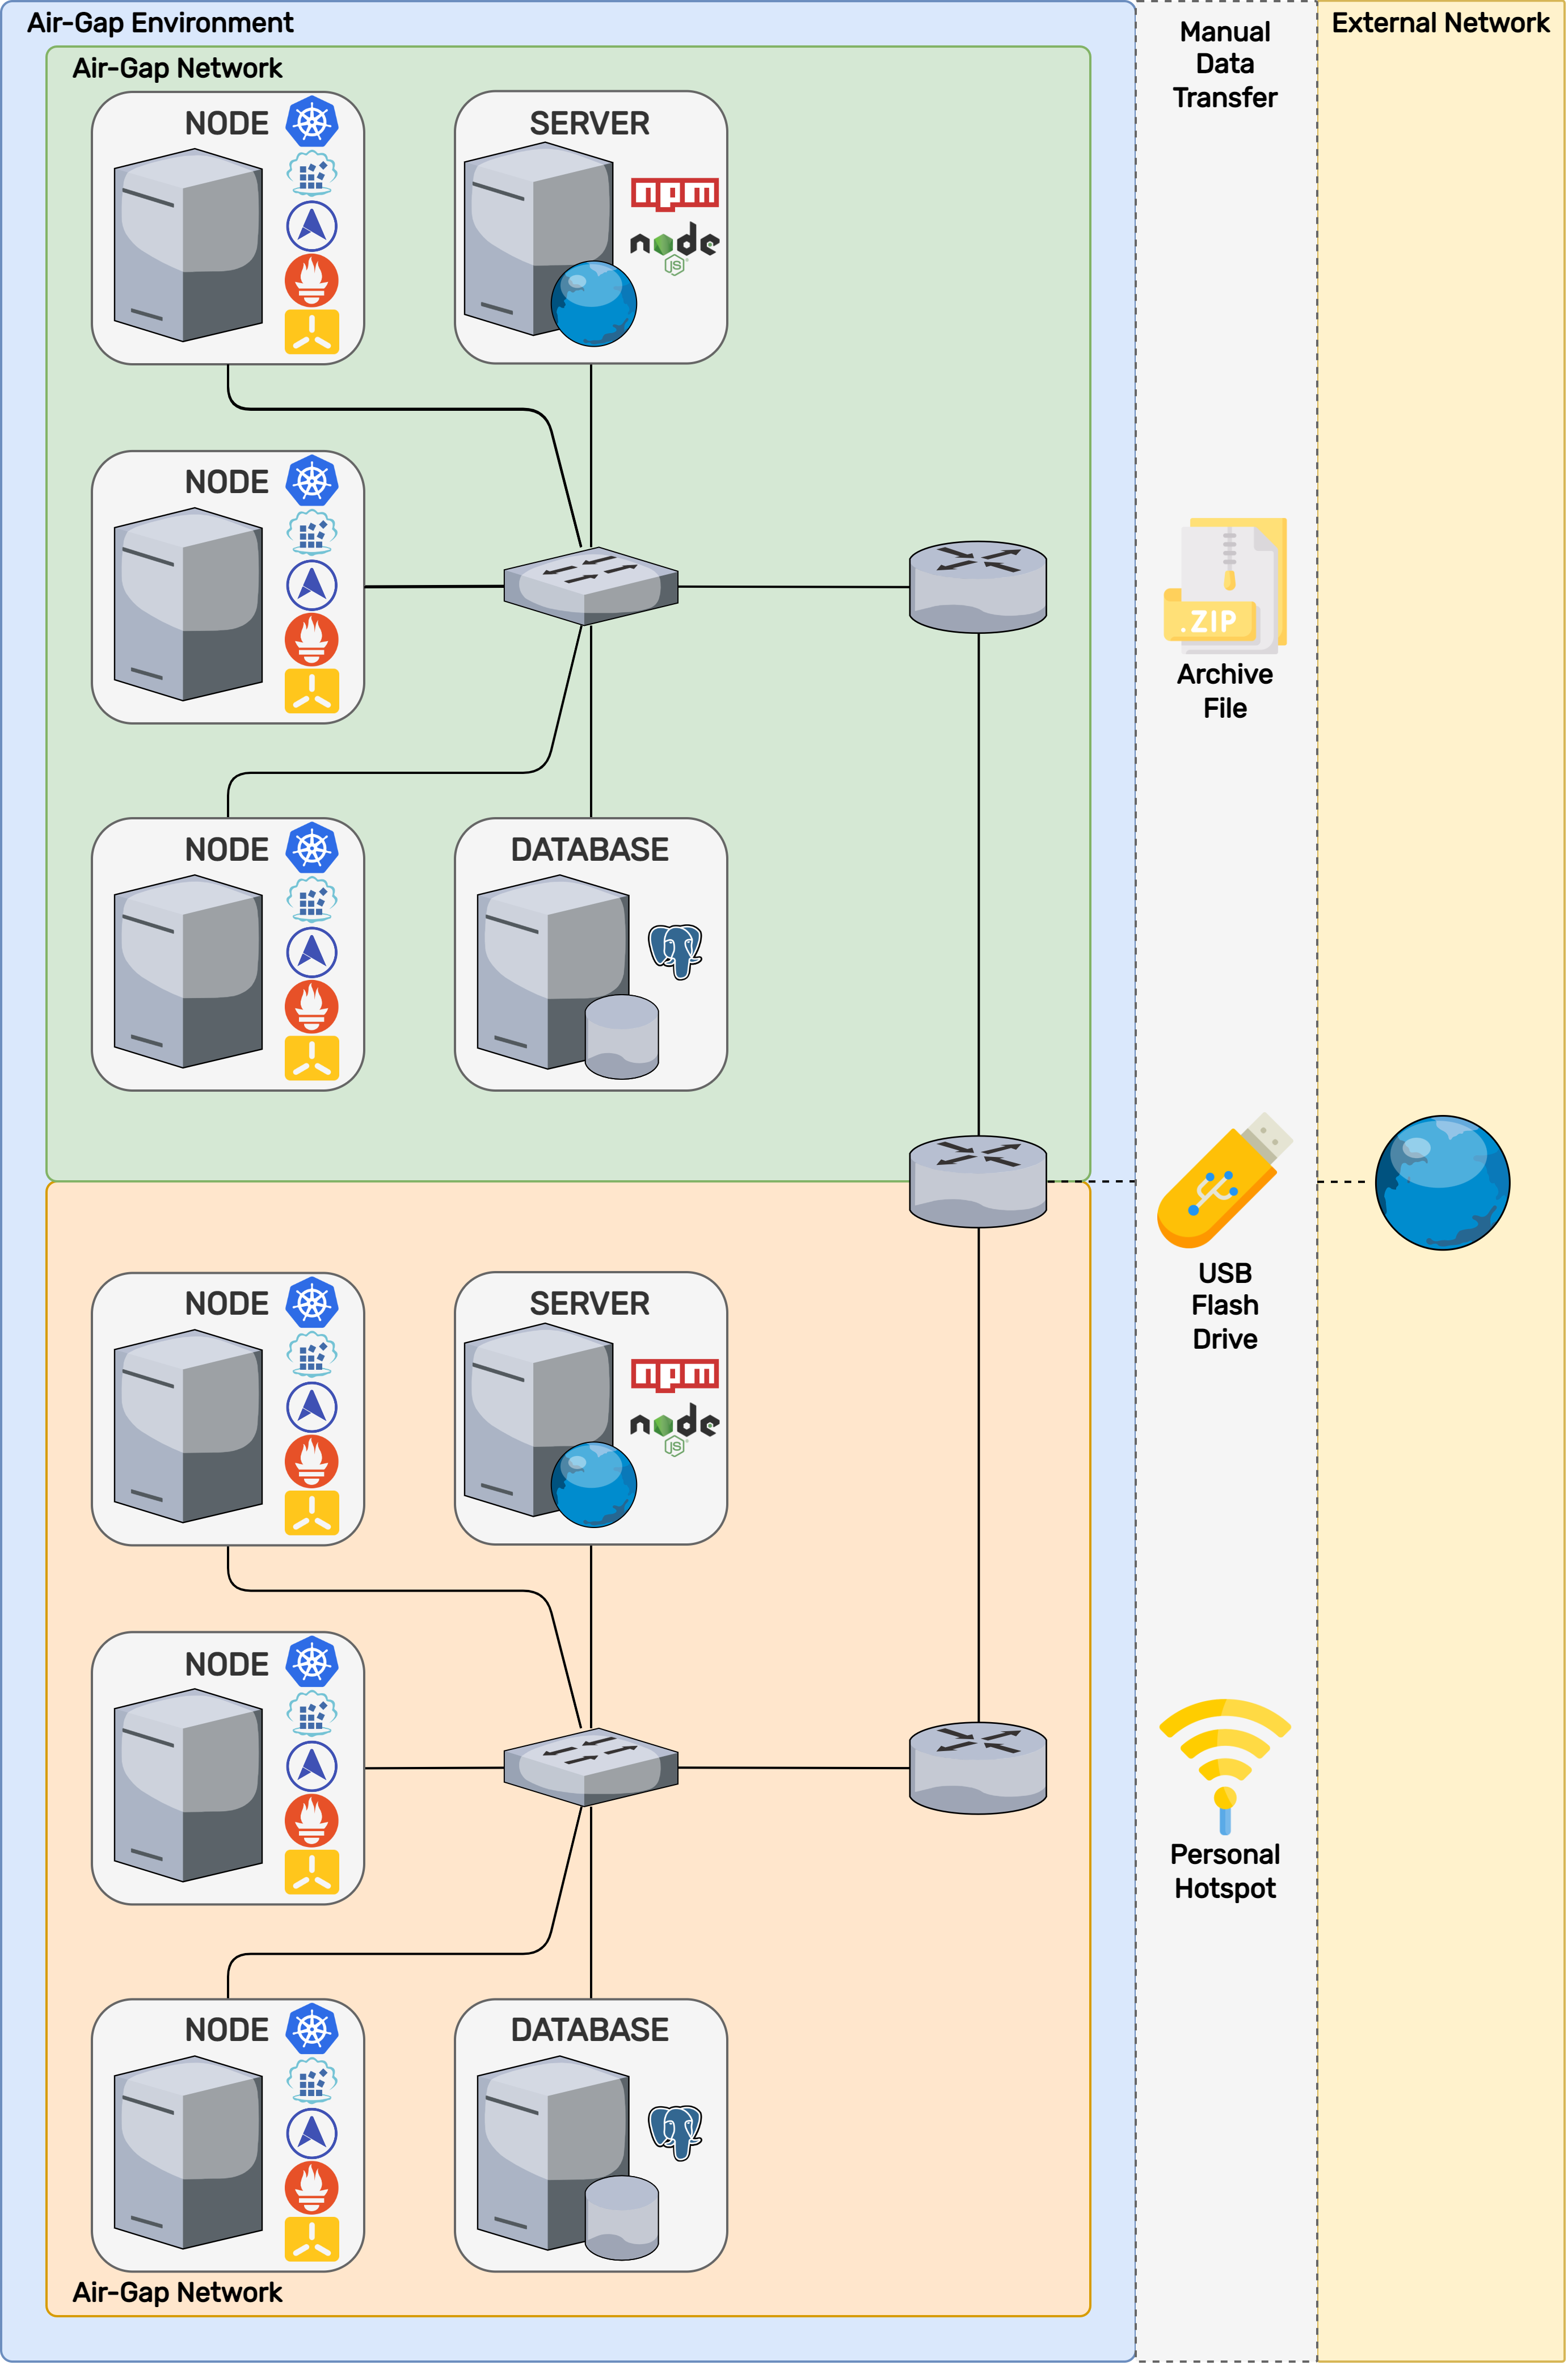
\includegraphics[width=.5\textwidth]{images/recluster/airgap.png}
  \caption{An
  Air-Gap
  Environment
  composed
  of
  two
  Air-Gap
  Networks
  that
  are
  physically
  and
  logically
  isolated
  by
  any
  external
  data
  exchange
  and
  network.}
  \label{fig:airgap}
\end{wrapfigure}

All devices in an Air-Gap environment have no physical connectivity to the public
internet or any other Local Area Network (LAN) that is not itself in an Air-Gap environment.
Email clients, browsers, SSH, and other communication applications are all physically
and logically isolated from the outside world. \\ %
Systems in an Air-Gap environment are permanently separated from the outside world
by default. However, if possible, the network can communicate with other
physically isolated devices. Any data transfer outside of the network must take place
via external hardware that is temporarily connected to the network. USB flash
drives, Hotspot devices and other removable media are examples of such hardware.
Importantly, these external devices must be physically connected to and disconnected
from the Air-Gap environment network by human intervention. \\ %
Figure \ref{fig:airgap} depicts an example overview of an Air-Gap environment consisting
of two distinct Air-Gap networks that can connect with one another. Because they
are on separate networks, each network resembles a hypothetical cluster implementation
where communication between the two does not directly involve cluster operations
and administration (see section
\ref{subsec:architecture_network_internal_network}). Every machine in the
environment is unable to exchange data, connect to any external network, or
connect to the internet in general. The only mechanism to move data between the Air-Gap
environment and the outside world is through the use of a USB flash drive, and
the only way to connect the Air-Gap networks to an external network and/or the
internet is through the use of a personal hotspot. Because no automated mechanisms
are involved, both of the latter actions need human interaction. \\ %
Air-Gap environments are frequently employed in Network Security scenarios where
security is a top priority. In an Air-Gap scenario, a correctly designed network
mandates that devices within the network be invisible to and successfully
isolated from remote threat actors, who often scan the public internet for vulnerable
devices. Similarly, an attacker outside of the Air-Gap environment network cannot
directly execute Remote Code Execution\footnote{\url{https://tuxcare.com/remote-code-execution-attack-what-it-is-how-to-protect-your-systems}}
(RCE) attacks on potential software vulnerabilities within the environment\cite{airgap}.
\\ %
Although Air-Gap environments are extensively employed in the security branch, high-security
scenarios are not the only ones for which the cluster implementation is designed.
In reality, there are situations in which the internet connection, and thus the
connectivity to the external global network is either too expensive to maintain
or not available at all in the location where the cluster is deployed. \\ %
To be fully compatible with an Air-Gap environment in various possible scenarios,
the cluster implementation is designed to have all external dependencies,
including custom Linux Distributions, pre-packaged with each cluster release and
without the need, by default, for possible external requests during its utilization.
As a result, all that is required is the unique archive file, which is
automatically created with each new release and contains all of the files
required to bootstrap a functioning cluster instance. Furthermore, even if not
in an Air-Gap environment, during the installation procedure, the organization
in charge of the cluster's administration can choose to either download all
external dependencies from the internet (every time for every node) or to
directly use the already available pre-packaged dependencies, reducing network usage
as well as overall installation time.

\subsection{K3s}
\label{subsec:implementation_dependencies_k3s}

\begin{wrapfigure}
  {l}{.25\textwidth} %
  \centering
  \def\stackalignment{l}\stackunder{ 
\includegraphics[width=\linewidth]{images/logos/k3s.png} } %
  {\scriptsize \parbox[t]{\linewidth}{ Source: \url{https://k3s.io}} }
  \caption{K3s logo}
\end{wrapfigure}

K3s is a lightweight Kubernetes distribution designed for production workloads in
resource-constrained, high-availability, unattended, and remote environments\cite{k3s}.
K3s is the cluster implementation's core, where all Kubernetes-related operations
are managed and processed. Because K3s is an element of both a Worker and a
Controller Node has no clear mapping to an architectural component. \\ %
K3s is distributed as a single small binary (less than 60MiB) that reduces the
requirements and procedures required to install, run, and automatically update a
production Kubernetes cluster\cite{k3s}. It is completely compatible with both
the \texttt{OpenRC} and \texttt{systemd} Init Systems (see section \ref{subsec:implementation_distributions_init_system})
and can run on any Linux distribution with a Kernel that satisfies the basic
Kubernetes requirements\footnote{\url{https://github.com/k3s-io/k3s/blob/master/install.sh}}.

\subsubsection{Enhancements}
\label{subsubsec:implementation_dependencies_k3s_enhancements}

K3s is a fully compliant Kubernetes distribution that has removed the majority of
legacy, alpha, and cloud-provider-specific code to minimize overall application size
and hardware requirements. Furthermore, K3s provides the following enhancements over
a conventional Kubernetes distribution\cite{k3s_enhancements}:
\begin{itemize}
  \item All required dependencies are pre-packaged within a single binary file,
    necessitating only a modern Kernel and \texttt{cgroup} mounts.

  \item Lightweight storage backend with \texttt{SQlite}\footnote{\url{https://www.sqlite.org}}
    as the default storage mechanism. Additional solutions based on \texttt{etcd}\footnote{\url{https://etcd.io}},
    \texttt{MySQL}\footnote{\url{https://www.mysql.com}}, or \texttt{PostgreSQL}
    are also available. Both embedded and external storage mechanisms are supported.
    \newline
    The cluster architecture design, as stated in chapter \ref{cha:architecture},
    is based on a high availability model rather than a fault tolerance strategy.
    As a result, it is recommended to use \texttt{etcd} (embedded or external) or
    the already available cluster's database as an external storage mechanism,
    eliminating needless data replications and relying on a single storage area
    that can be controlled autonomously.

  \item Secure by default, with appropriate default parameters for lightweight
    environments. K3s manages automatically the complexity of TLS\footnote{\url{https://wikipedia.org/wiki/Transport_Layer_Security}}
    (Transport Layer Security) like certificate distributions.
    \newline
    If security is not a priority, or if the cluster is in an Air-Gap environment,
    the security settings can be relaxed to increase overall cluster's
    performance while simultaneously decreasing resource utilization.
\end{itemize}

\subsubsection{Architecture}
\label{subsubsec:implementation_dependencies_k3s_architecture}

K3s architecture clearly distinguishes between two types of Nodes, Server nodes
and Agent nodes, which are described below\cite{k3s_architecture}. Furthermore,
figure \ref{fig:k3s} depicts the distinction between the two node types by
displaying the various components provided on each node.
\begin{enumerate}
  \item \texttt{Server} node
    \newline
    A server node is defined as a host running the K3s server command (\lstinline[language=shell,
    basicstyle=\ttfamily, morekeywords={[2]{k3s}}, morekeywords={[3]{server}}]{k3s server}),
    with K3s managing the control-plane and datastore components.
    \newline
    The \texttt{Controller} Node component of the cluster's architecture, depicted
    in the section \ref{subsubsec:architecture_components_node_controller}, is a
    logical mapping to the K3s Server Node.

  \item \texttt{Agent} node
    \newline
    An agent node is defined as a host running the K3s agent command (\lstinline[language=shell,
    basicstyle=\ttfamily, morekeywords={[2]{k3s}}, morekeywords={[3]{agent}}]{k3s agent}),
    that does not have any datastore or control-plane components running.
    \newline
    The \texttt{Worker} Node component of the cluster's architecture, depicted in
    the section \ref{subsubsec:architecture_components_node_worker}, is a
    logical mapping to the K3s Agent Node.
\end{enumerate}
\begin{figure}[htbp]
  \centering
  \def\stackalignment{r}\stackunder{ 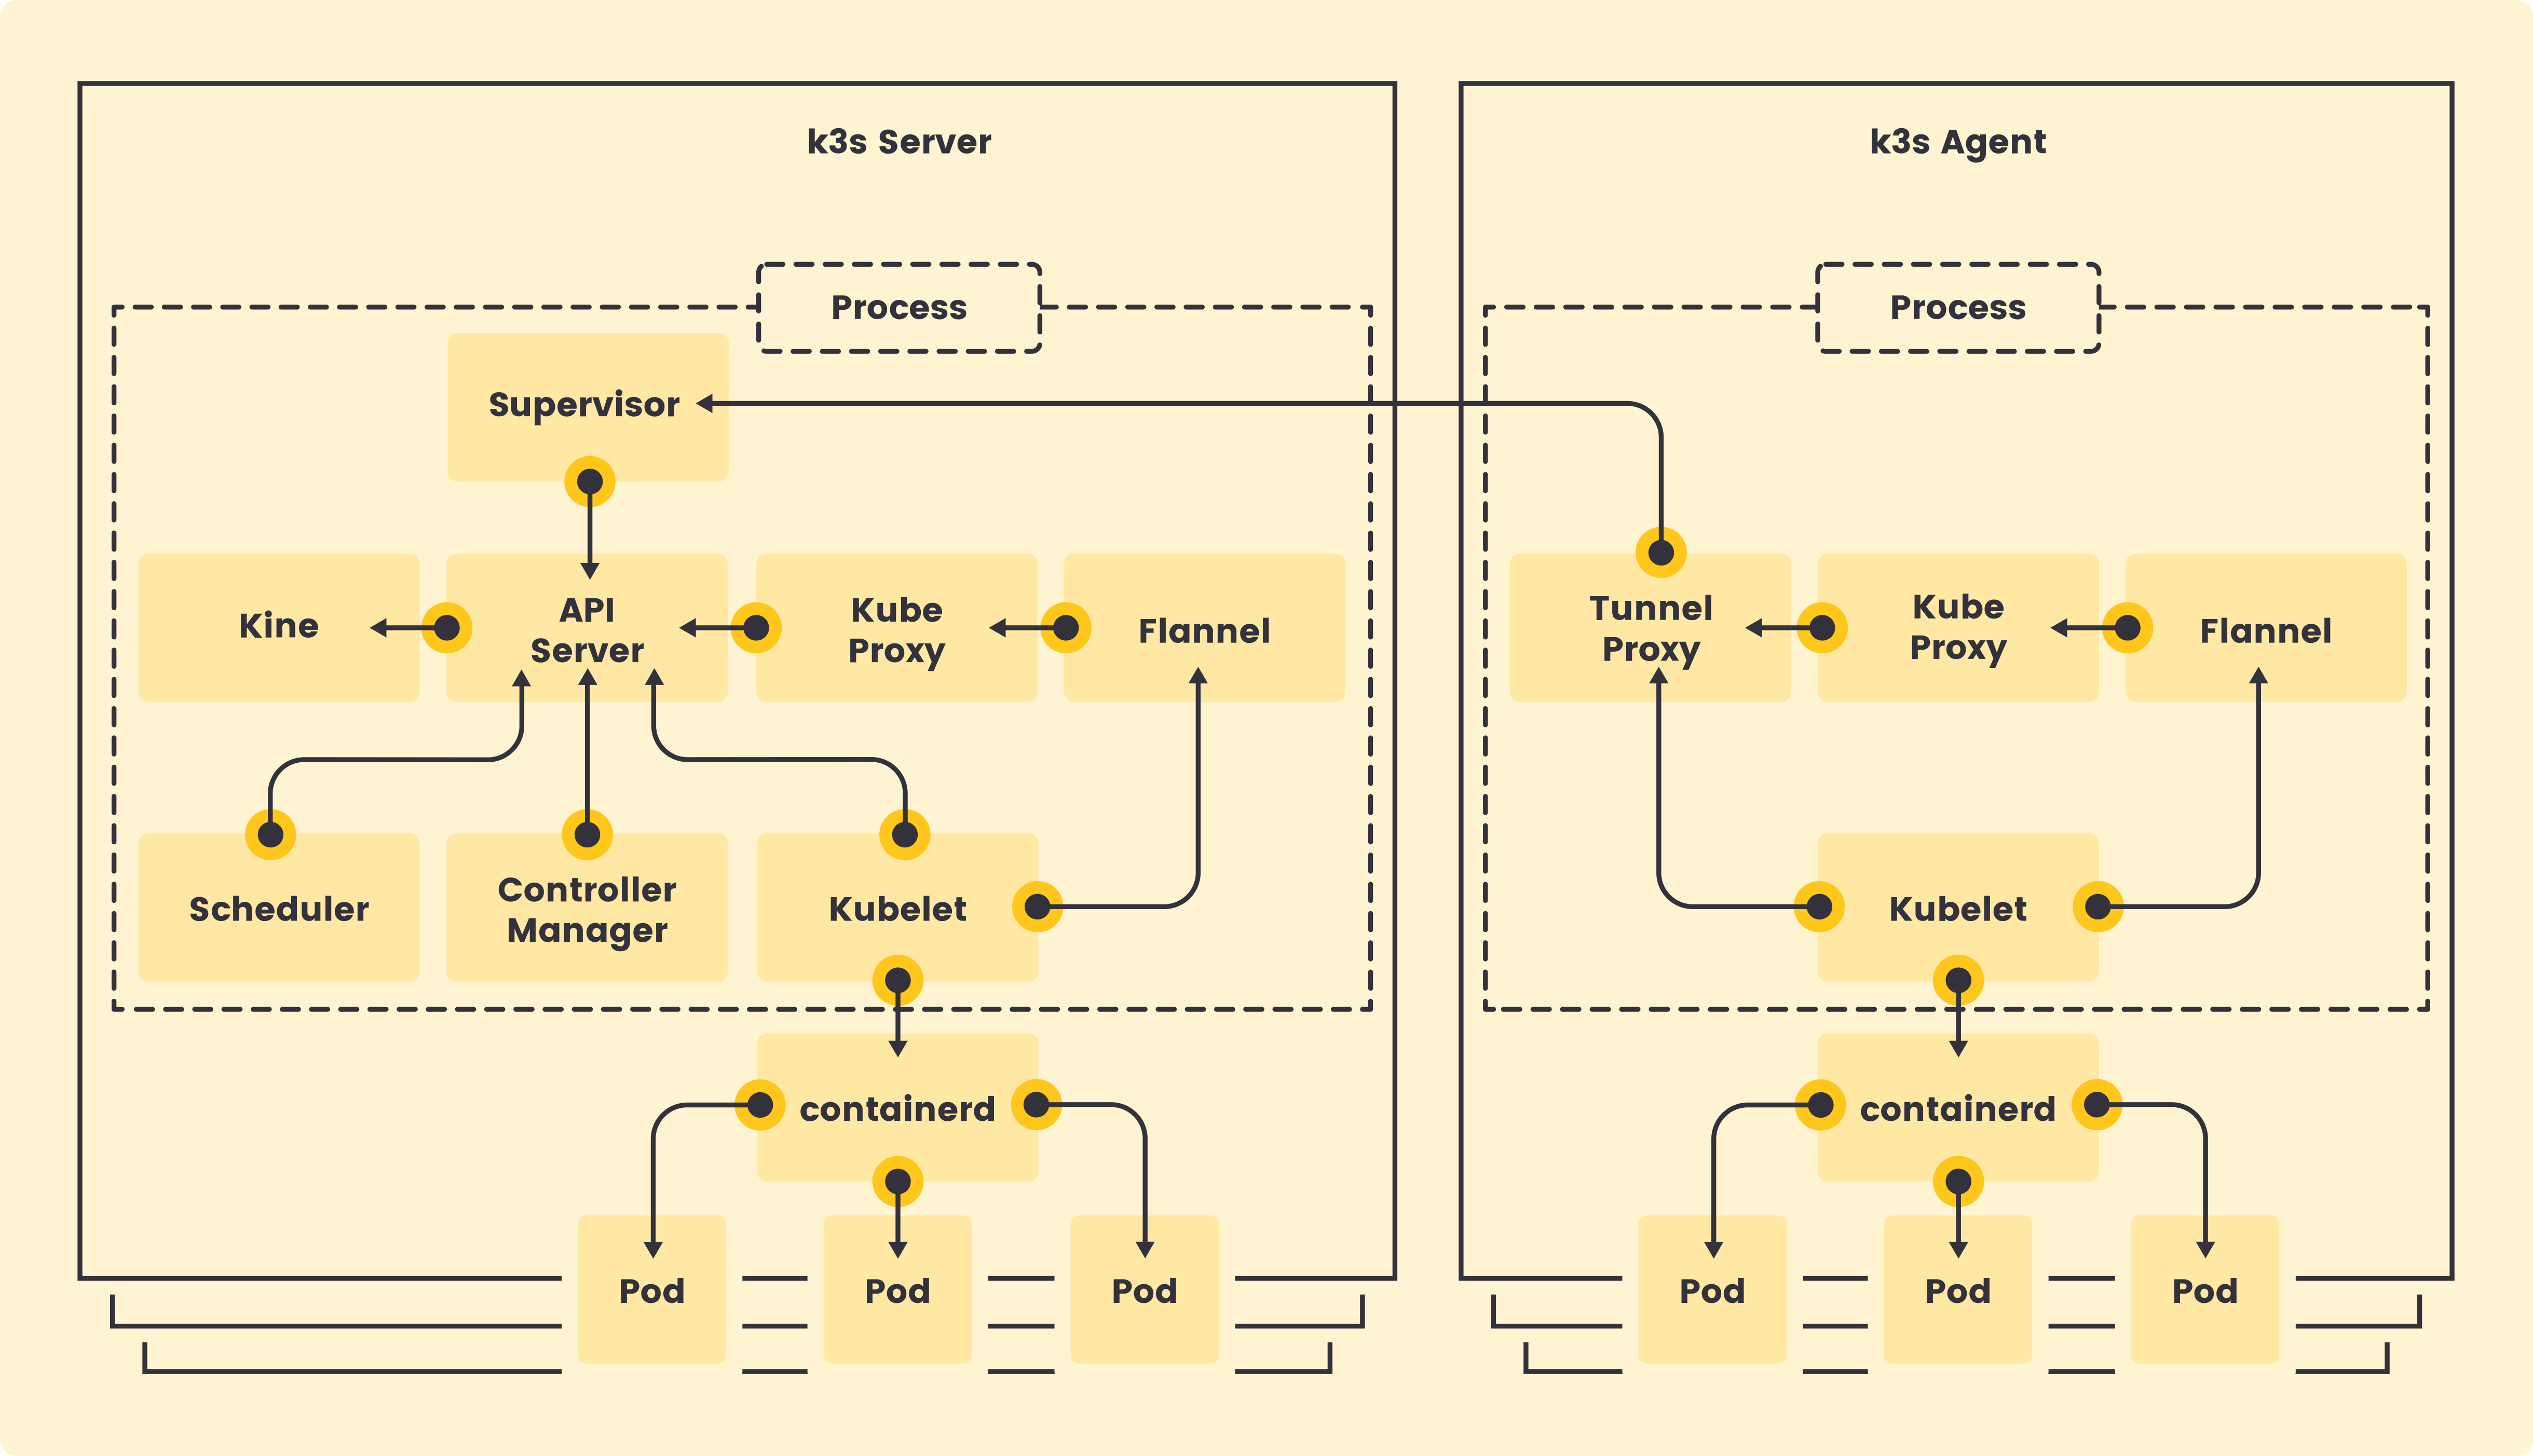
\includegraphics[width=.9\linewidth]{images/recluster/k3s.png} } %
  {\scriptsize Source: \url{https://k3s.io} }
  \caption{Difference between K3s Server and K3s Agent nodes}
  \label{fig:k3s}
\end{figure}
Additionally, the K3s architecture is completely adaptable and may accommodate a
variety of different setups, as shown in the list below, depending on the
cluster's usage and ultimate goal\cite{k3s_architecture}.
\begin{enumerate}
  \item \texttt{Single Server with an Embedded Database}
    \newline
    A single-node K3s server with a \texttt{SQLite} database embedded. Each
    agent node is associated with the same K3s Server node. By utilizing the K3s
    API on the Server node, an administrator can directly control the Kubernetes
    resources.
    \newline
    This configuration is only recommended for testing purposes, not for real-world
    production deployments or cluster implementation.

  \item \texttt{High-Availability Server with an Embedded Database}
    \newline
    An High-Availability (HA) K3s cluster is composed of two or more Server
    nodes that serve the Kubernetes API as well as additional control plane
    services. The database is embedded and operated on the same Server node by the
    K3s instance.

  \item \texttt{High-Availability Server with an External Database}
    \newline
    Similar to the previous setup, however, the datastore is located outside of
    the Server Node. The K3s Server instance does not execute any database application
    and instead relies on an externally accessible and operating database.
\end{enumerate}

\subsubsection{The Choice}
\label{subsubsec:implementation_dependencies_k3s_the_choice}

The K3s distribution was chosen from among a multitude of various Kubernetes
distributions, including the official one, for the four main reasons, listed below.

\begin{enumerate}
  \item Minimal hardware requirements that are simple to satisfy, even on older
    systems\cite{k3s_hardware}:
    \begin{itemize}
      \item A Server node requires 1 GiB of memory and 1 CPU core.
        \newline
        As stated in the section
        \ref{subsubsec:architecture_components_node_controller}, the Server (Controller)
        node's minimal hardware requirements must be adjusted to match the cluster's
        size. A cluster with hundreds of Worker nodes managed by a single Server
        node with only 1 GiB of memory and 1 CPU core is unrealistic.

      \item An Agent node requires 512 MiB of memory and 1 CPU core.
        \newline
        A Raspberry Pi 3 Model B single-board computer, released in February 2016\footnote{\url{https://www.raspberrypi.com/products/raspberry-pi-3-model-b-plus}}
        (7 years ago at the time of writing), is fully compatible with K3s and
        can operate as a Worker node without any difficulty.
    \end{itemize}
    In comparison, the official Kubernetes distribution, \texttt{kubeadm},
    necessitates at least 2 GiB of memory and 2 CPU cores\cite{k8s_hardware}.

  \item Configurability, modularity, and usability\cite{k3s_configuration}.
    \newline
    As an example, it is extremely simple to bootstrap a small Kubernetes
    cluster using K3s in a Single Server with an Embedded Database setup:
    \begin{itemize}
      \item Start the Server node with a unique token (used to join a Server or
        Agent nodes to the cluster).
        \newline
        \lstinline[language=shell, alsoletter={-}, morekeywords={[2]{k3s}}, morekeywords={[3]{--token}},
        morekeywords={[4]{server}}, xleftmargin=\parindent]{ k3s server --token "<TOKEN>"}

      \item Start the Agent node specifying the unique token and the Server address.
        \newline
        \lstinline[language=shell, alsoletter={-}, morekeywords={[2]{k3s}}, morekeywords={[3]{--token, --server}},
        morekeywords={[4]{agent}}, xleftmargin=\parindent]{ k3s agent --token "<TOKEN>" --server "<SERVER_ADDRESS>"}
    \end{itemize}

  \item K3s can be easily installed in an Air-Gap environment. The only
    additional steps necessary to have a fully functional cluster in comparison
    to a standard installation are the deployment of a private registry (see section
    \ref{subsec:implementation_dependencies_docker_registry}) and the manual
    deployment of particular container images on each node\cite{k3s_airgap}.
    \newline
    By default, the cluster implementation installation (see section
    \ref{sec:implementation_installer}) already meets the latter two requirements.
    As a result, an organization that has to deploy a cluster in an Air-Gap environment
    already has received all of the required files and programs without the need
    for any additional data transfer involving an internet connection. As a
    result, an organization that has to deploy a cluster in an Air-Gap environment
    already has all of the necessary files and applications without the need for
    any additional data transfer involving an internet connection.

  \item On August 19th, 2020, the K3s project was approved into the Cloud Native
    Computing Foundation\footnote{\url{https://www.cncf.io}} (CNCF) with Sandbox
    maturity level\cite{cncf_k3s}. CNCF is a vendor-neutral cloud native computing,
    hosting critical components of the global technology infrastructure
    dedicated to making cloud native ubiquitous\cite{cncf}. CNCF certifies
    Kubernetes software compliance, ensuring that every vendor's version of Kubernetes,
    as well as open source community versions, supports the large set of Kubernetes
    APIs\cite{cncf_conformance}. The latter means full compatibility with all existing
    Kubernetes products and software, allowing for the interchangeability of
    various components within the cluster implementation representing diverse
    organizations' core aspects.
\end{enumerate}

\subsection{Node Exporter}
\label{subsec:implementation_dependencies_node_exporter}

Node Exporter provides hardware and OS-related metrics exposed by the \texttt{*NIX}
Kernel\cite{node_exporter}. It is widely used in both testing and production environments
thanks to its broad compatibility, simplicity of configuration, and reliability,
and it can be regarded as the reference implementation for a Metrics Server. Because
it is an element that constitutes both a Worker and a Controller Node, Node
Exporter does not have a clear mapping to an architectural component.

\subsubsection{Collectors}
\label{subsubsec:implementation_dependencies_node_exporter-collectors}

For each Operating System, such as Linux or OpenBSD\footnote{\url{https://www.openbsd.org}},
Node Exporter supports a wide range of different collectors, such as \texttt{cpu}
for providing CPU statistics or \texttt{meminfo} for exposing memory statistics\footnote{\url{https://github.com/prometheus/node_exporter\#collectors}}.
A collector is an element of an exporter, which represents a collection of
metrics. If it is part of direct instrumentation, it may be a single metric, or it
may be multiple metrics if it is pulling metrics from another system\cite{prometheus_metrics}.
Collectors can be enabled (\lstinline[language=shell, basicstyle=\ttfamily,
alsoletter={_, -, ., <, >}, morekeywords={[2]{node_exporter}}, morekeywords={[3]{--collector.<NAME>}}]{node_exporter --collector.<NAME>})
or disabled (\lstinline[language=shell, basicstyle=\ttfamily, alsoletter={_, -, ., <, >},
morekeywords={[2]{node_exporter}}, morekeywords={[3]{--no-collector.<NAME>}}]{node_exporter --no-collector.<NAME>})
based on the data that the node needs to provide for monitoring. The exposed
metrics are represented in a standardized format (see section \ref{subsubsec:implementation_dependencies_prometheus_features}),
allowing Prometheus (see section
\ref{subsec:implementation_dependencies_prometheus}) to analyze and process them.
Listing \ref{lst:node_exporter} depicts an example section of a response
generated by Node Exporter running on a node with two CPU cores and
approximately 4 GiB of system memory. Three metrics are displayed, one from the
\texttt{cpu} collector and the other two from the \texttt{meminfo} collector: \texttt{node\_cpu\_seconds\_total}
is a counter that keeps track of how many seconds each CPU core (\texttt{0} and
\texttt{1}) spent in each mode, \texttt{node\_memory\_MemTotal\_bytes} is the
total amount of physical memory (in bytes), and \texttt{node\_memory\_MemFree\_bytes}
is the total amount of physical memory (in bytes) that is not in use.

\begin{lstlisting}[language=prometheus, xleftmargin=\parindent, alsoletter={_}, morekeywords={node_cpu_seconds_total, node_memory_MemTotal_bytes, node_memory_MemFree_bytes}, morekeywords={[2]{cpu, mode}}, label={lst:node_exporter}, caption=Example section of a Node Exporter response with \texttt{cpu} and \texttt{meminfo} collectors enabled]
  # HELP node_cpu_seconds_total Seconds the CPUs spent in each mode.
  # TYPE node_cpu_seconds_total counter
  node_cpu_seconds_total{cpu="0",mode="idle"} 980.6
  node_cpu_seconds_total{cpu="0",mode="iowait"} 2.18
  node_cpu_seconds_total{cpu="0",mode="irq"} 2.97
  node_cpu_seconds_total{cpu="0",mode="nice"} 0
  node_cpu_seconds_total{cpu="0",mode="softirq"} 1.47
  node_cpu_seconds_total{cpu="0",mode="steal"} 0
  node_cpu_seconds_total{cpu="0",mode="system"} 0.59
  node_cpu_seconds_total{cpu="0",mode="user"} 423.57
  node_cpu_seconds_total{cpu="1",mode="idle"} 954.29
  node_cpu_seconds_total{cpu="1",mode="iowait"} 4.44
  node_cpu_seconds_total{cpu="1",mode="irq"} 0.98
  node_cpu_seconds_total{cpu="1",mode="nice"} 0
  node_cpu_seconds_total{cpu="1",mode="softirq"} 1.94
  node_cpu_seconds_total{cpu="1",mode="steal"} 0
  node_cpu_seconds_total{cpu="1",mode="system"} 1.43
  node_cpu_seconds_total{cpu="1",mode="user"} 448.79
  # HELP node_memory_MemTotal_bytes Memory information field MemTotal_bytes.
  # TYPE node_memory_MemTotal_bytes gauge
  node_memory_MemTotal_bytes 4.063023104e+09
  # HELP node_memory_MemFree_bytes Memory information field MemFree_bytes.
  # TYPE node_memory_MemFree_bytes gauge
  node_memory_MemFree_bytes 1.88204544e+09
\end{lstlisting}

\subsubsection{Installer}
\label{subsubsec:implementation_dependencies_node_exporter_installer}

To represent diverse organizations' goals and preferences, the cluster's
installation procedure on a system node, as detailed in the section \ref{sec:implementation_installer},
requires complete automation and configuration when installing a dependency. Despite
being a very popular and widely used application, Node Exporter lacks a fully
featured installation script, such as \texttt{install.sh}\footnote{\url{https://github.com/k3s-io/k3s/blob/master/install.sh}}
provided by K3s, which can simply automate every operation. As a solution, a side
project called Node Exporter Installer was established to address the latter issue(s).
The installation script is completely POSIX-compliant, highly customizable, \texttt{OpenRC}
and \texttt{systemd} Init Systems compatible, and requires only basic
applications as dependencies that are ubiquitous in almost all \texttt{*NIX}
systems. The project is completely Open Source, and other users may use it to
easily and rapidly configure and install Node Exporter. Attachment \ref{sec:corollary_projects_node_exporter_installer}
has a detailed description of the Node Exporter Installer project.

\subsubsection{Graphics Processing Unit metrics}
\label{subsubsec:implementation_dependencies_node_exporter_graphics_processing_unit_metrics}

Node Exporter does not support exporting Graphics Processing Unit\footnote{\url{https://wikipedia.org/wiki/Graphics_processing_unit}}
(GPU) metrics. In general, supporting systems equipped with GPU(s) in a uniform and
easily accessible manner is a fairly hard undertaking that necessitates a significant
amount of work in terms of initial setup and overall administration. Furthermore,
GPU-equipped systems require availability and compatibility with a per GPU model-specific
Kernel driver to be efficient without scarifying precious performance and wasting
resources. Nevertheless, exporter implementations such as \texttt{DCGM-Exporter}\footnote{\url{https://github.com/NVIDIA/dcgm-exporter}}
and \texttt{nvidia\_gpu\_exporter}\footnote{\url{https://github.com/utkuozdemir/nvidia_gpu_exporter}}
are specifically designed to provide just GPU metrics that can be used alongside
Node Exporter metrics. However, all current GPU exporters only support NVIDIA\footnote{\url{https://www.nvidia.com}}
GPUs and require extra dependencies to be deployed. Moreover, because of its intrinsic
heterogeneity, purpose, and complexity of supporting GPU systems, the cluster
implementation currently does not offer any GPU data, metrics, or statistics. Furthermore,
because the cluster is primarily composed of consumer hardware rather than high-end
enterprise solutions, there is a high possibility that some systems would be equipped
with AMD\footnote{\url{https://www.amd.com}} GPUs, which, as previously stated,
are currently not supported by any official and/or reliable exporter program.

\subsection{Docker Registry}
\label{subsec:implementation_dependencies_docker_registry}

\begin{wrapfigure}
  {l}{.25\textwidth} %
  \centering
  \def\stackalignment{l}\stackunder{ 
\includegraphics[width=\linewidth]{images/logos/docker_registry.png} } %
  {\scriptsize \parbox[t]{\linewidth}{ Source: \url{https://github.com/distribution/distribution}} }
  \caption{Docker Registry logo}
\end{wrapfigure}

Docker Registry is a stateless, highly scalable server-side service for storing and
distributing container-based application images\cite{docker_registry}. A registry
is a storage and content delivery system that holds container images in different
tagged versions\cite{docker_registry_about}. \\ %
The Docker Registry, thus the name, has a direct mapping to the Registry
component of the cluster architecture.

\subsubsection{Image Naming}
\label{subsubsec:implementation_dependencies_docker_registry_image_naming}

\texttt{[REGISTRY\_HOSTNAME][:REGISTRY\_PORT]IMAGE[:TAG]} \\ %
An image name is made up of slash-separated name fields that are optionally
prefixed with a registry hostname, complying with standard DNS\footnote{\url{https://wikipedia.org/wiki/Domain_Name_System}}
(Domain Name System) rules, and optionally postfixed with a tag name that
identifies different versions of the same series of images. If a hostname is specified,
it may be followed by a port number in the format \texttt{:PORT}. If the registry
hostname is not provided, Docker, Kubernetes, Podman, and practically every other
software that deals with container images by default utilizes Docker's public registry
(Docker Hub\footnote{\url{https://hub.docker.com}}, which is hosted at \texttt{docker.io}
at port \texttt{443})\cite{k8s_image_names}. If no tag name is supplied, the value
\texttt{latest} is automatically assigned, indicating that the image is designated
as the most recent available release version\cite{docker_tag}. \\ %
For example, the image name \texttt{node:18} (short for \texttt{docker.io:443/node:18})
indicates the container image of Node.js version 18 accessible on the Docker public
registry at port \texttt{443}. Instead, the name \texttt{registry.recluster.local:5000/node:18}
also identifies the container image of Node.js version 18 but available on the local
private registry \texttt{registry.recluster.local} at port \texttt{5000}.
Therefore, if there is a requirement in the cluster to refer to container images
on a registry different from the default one, the full image name must be
provided.

\subsubsection{Hostname To IP Address Mapping}
\label{subsubsec:implementation_dependencies_docker_registry_hostname_to_ip_address_mapping}

A local registry deployment requires that there be a known mapping in the cluster
between the registry hostname and the IP address where the registry instance is executing.
There are three options available, as indicated in the list below:
\begin{enumerate}
  \item Use a custom Kubernetes distribution configuration file/entry to instruct
    the container runtime about the mapping. Moreover, if the Kubernetes distribution
    and runtime support it, the mapping may also be used to rewrite the default
    Docker Hub registry hostname to link to an alternative local registry
    hostname. An example image \texttt{docker.io/node:18} is transparently
    rewritten as \texttt{registry.recluster.local:5000/node:18}. The latter, allows
    the cluster to continue operating without any changes to the container image
    name of the deployments, enabling future less possible maintenance burden
    because the only change that has to be performed is on the configuration
    file and not on the cluster deployments.
    \newline
    This functionality is supported by default in K3s through a configuration file
    called \texttt{registries.yaml} that must be saved in the directory \texttt{/etc/rancher/k3s}
    on each node in the Kubernetes cluster\footnote{\url{https://docs.k3s.io/installation/private-registry}}.

  \item Add an entry to the \texttt{/etc/hosts}\footnote{\url{https://tldp.org/LDP/solrhe/Securing-Optimizing-Linux-RH-Edition-v1.3/chap9sec95.html}}
    file on each cluster node.

  \item Deploy a DNS component that must be operational in the cluster at all times.
    \newline
    This solution requires that all cluster nodes be configured to know about
    the local DNS, either manually by modifying \texttt{/etc/resolv.conf}\footnote{\url{https://tldp.org/LDP/nag/node84.html}}
    file or automatically via DHCP\footnote{\url{https://wikipedia.org/wiki/Dynamic_Host_Configuration_Protocol}}
    (Dynamic Host Configuration Protocol).
\end{enumerate}
Each of the three options has pros and cons. If the cluster size is relatively small
and the IP address of the local registry does not vary over time, the first or
second (depending on whether the chosen Kubernetes distribution supports the functionality)
solutions are recommended. However, if the cluster consists of numerous nodes, or
if the IP address of the registry changes regularly, or if further hostname to
IP mappings are required, then having a DNS component is by far the best approach.
Nonetheless, the organization operating the cluster makes the final decision on what
is the best solution: nothing prevents the deployment of a DNS component even in
a very small cluster. \\ %
Because reCluster is based on K3s, has a modest number of nodes, and the IP
address of the registry never changes thanks to MetalLB (see section \ref{subsec:implementation_dependencies_metallb}),
the decision fell almost naturally on the first alternative. Section
\ref{subsec:implementation_installer_configuration_files} goes into further
detail on this.

\subsubsection{Image Storage}
\label{subsubsec:implementation_dependencies_docker_registry_image_storage}

The registry must store the available container images in persistent storage in order
to keep them if a failure occurs or the registry instance is restarted. Storage
operation and management are not handled by the registry itself but are
delegated to specialized drivers, the default driver of which is the local POSIX
file system of the node executing the registry instance\cite{docker_registry_about}.
\\ %
Saving all container images on a single node is considered bad practice since it
creates a single point of failure that might result in the loss of all images. Therefore,
the cluster should be equipped with extra and more powerful storage drivers
intended to tolerate multiple storage device failures at the same time as well
as automated data recovery. It should be noted, however, that the driver(s)
chosen must be compatible with the cluster environment, nodes hardware, and/or
meet certain extra requirements. Almost every cloud provider supplies its customized
driver that is compatible with the underlying high-performance and distributed data
center storage system. Implementing a custom storage driver for the cluster
implementation that meets all of the above requirements is extremely difficult
owing to the overall complexity. Thankfully, a storage driver, Longhorn, from
the same creators of K3s, already exists to address the latter with extra features
and customization. Thankfully, a storage driver that addresses the latter problem
with extra features and customization already exists: Longhorn, developed by the
same team that created K3s. \\ %
Longhorn\footnote{\url{https://longhorn.io}} is an Open Source and CNCF Incubating
project\footnote{\url{https://www.cncf.io/projects/longhorn}} that provides a lightweight,
reliable, and simple distributed block storage system for Kubernetes\cite{longhorn}.
A block storage system stores data in fixed-size blocks, with each block
identified by a memory address\cite{block_storage}. Longhorn provides a
dedicated storage controller for each volume and replicates it synchronously
across multiple replicas stored on multiple nodes. Kubernetes is used to orchestrate
and manage the storage controller and replicas\cite{longhorn_architecture}. Figure
\ref{fig:longhorn} depicts Longhorn's architecture overview and Read/Write Data Flow
between the Volume, Longhorn Engine, Replica Instances, and Disks.
\begin{figure}[htbp]
  \centering
  \def\stackalignment{r}\stackunder{ 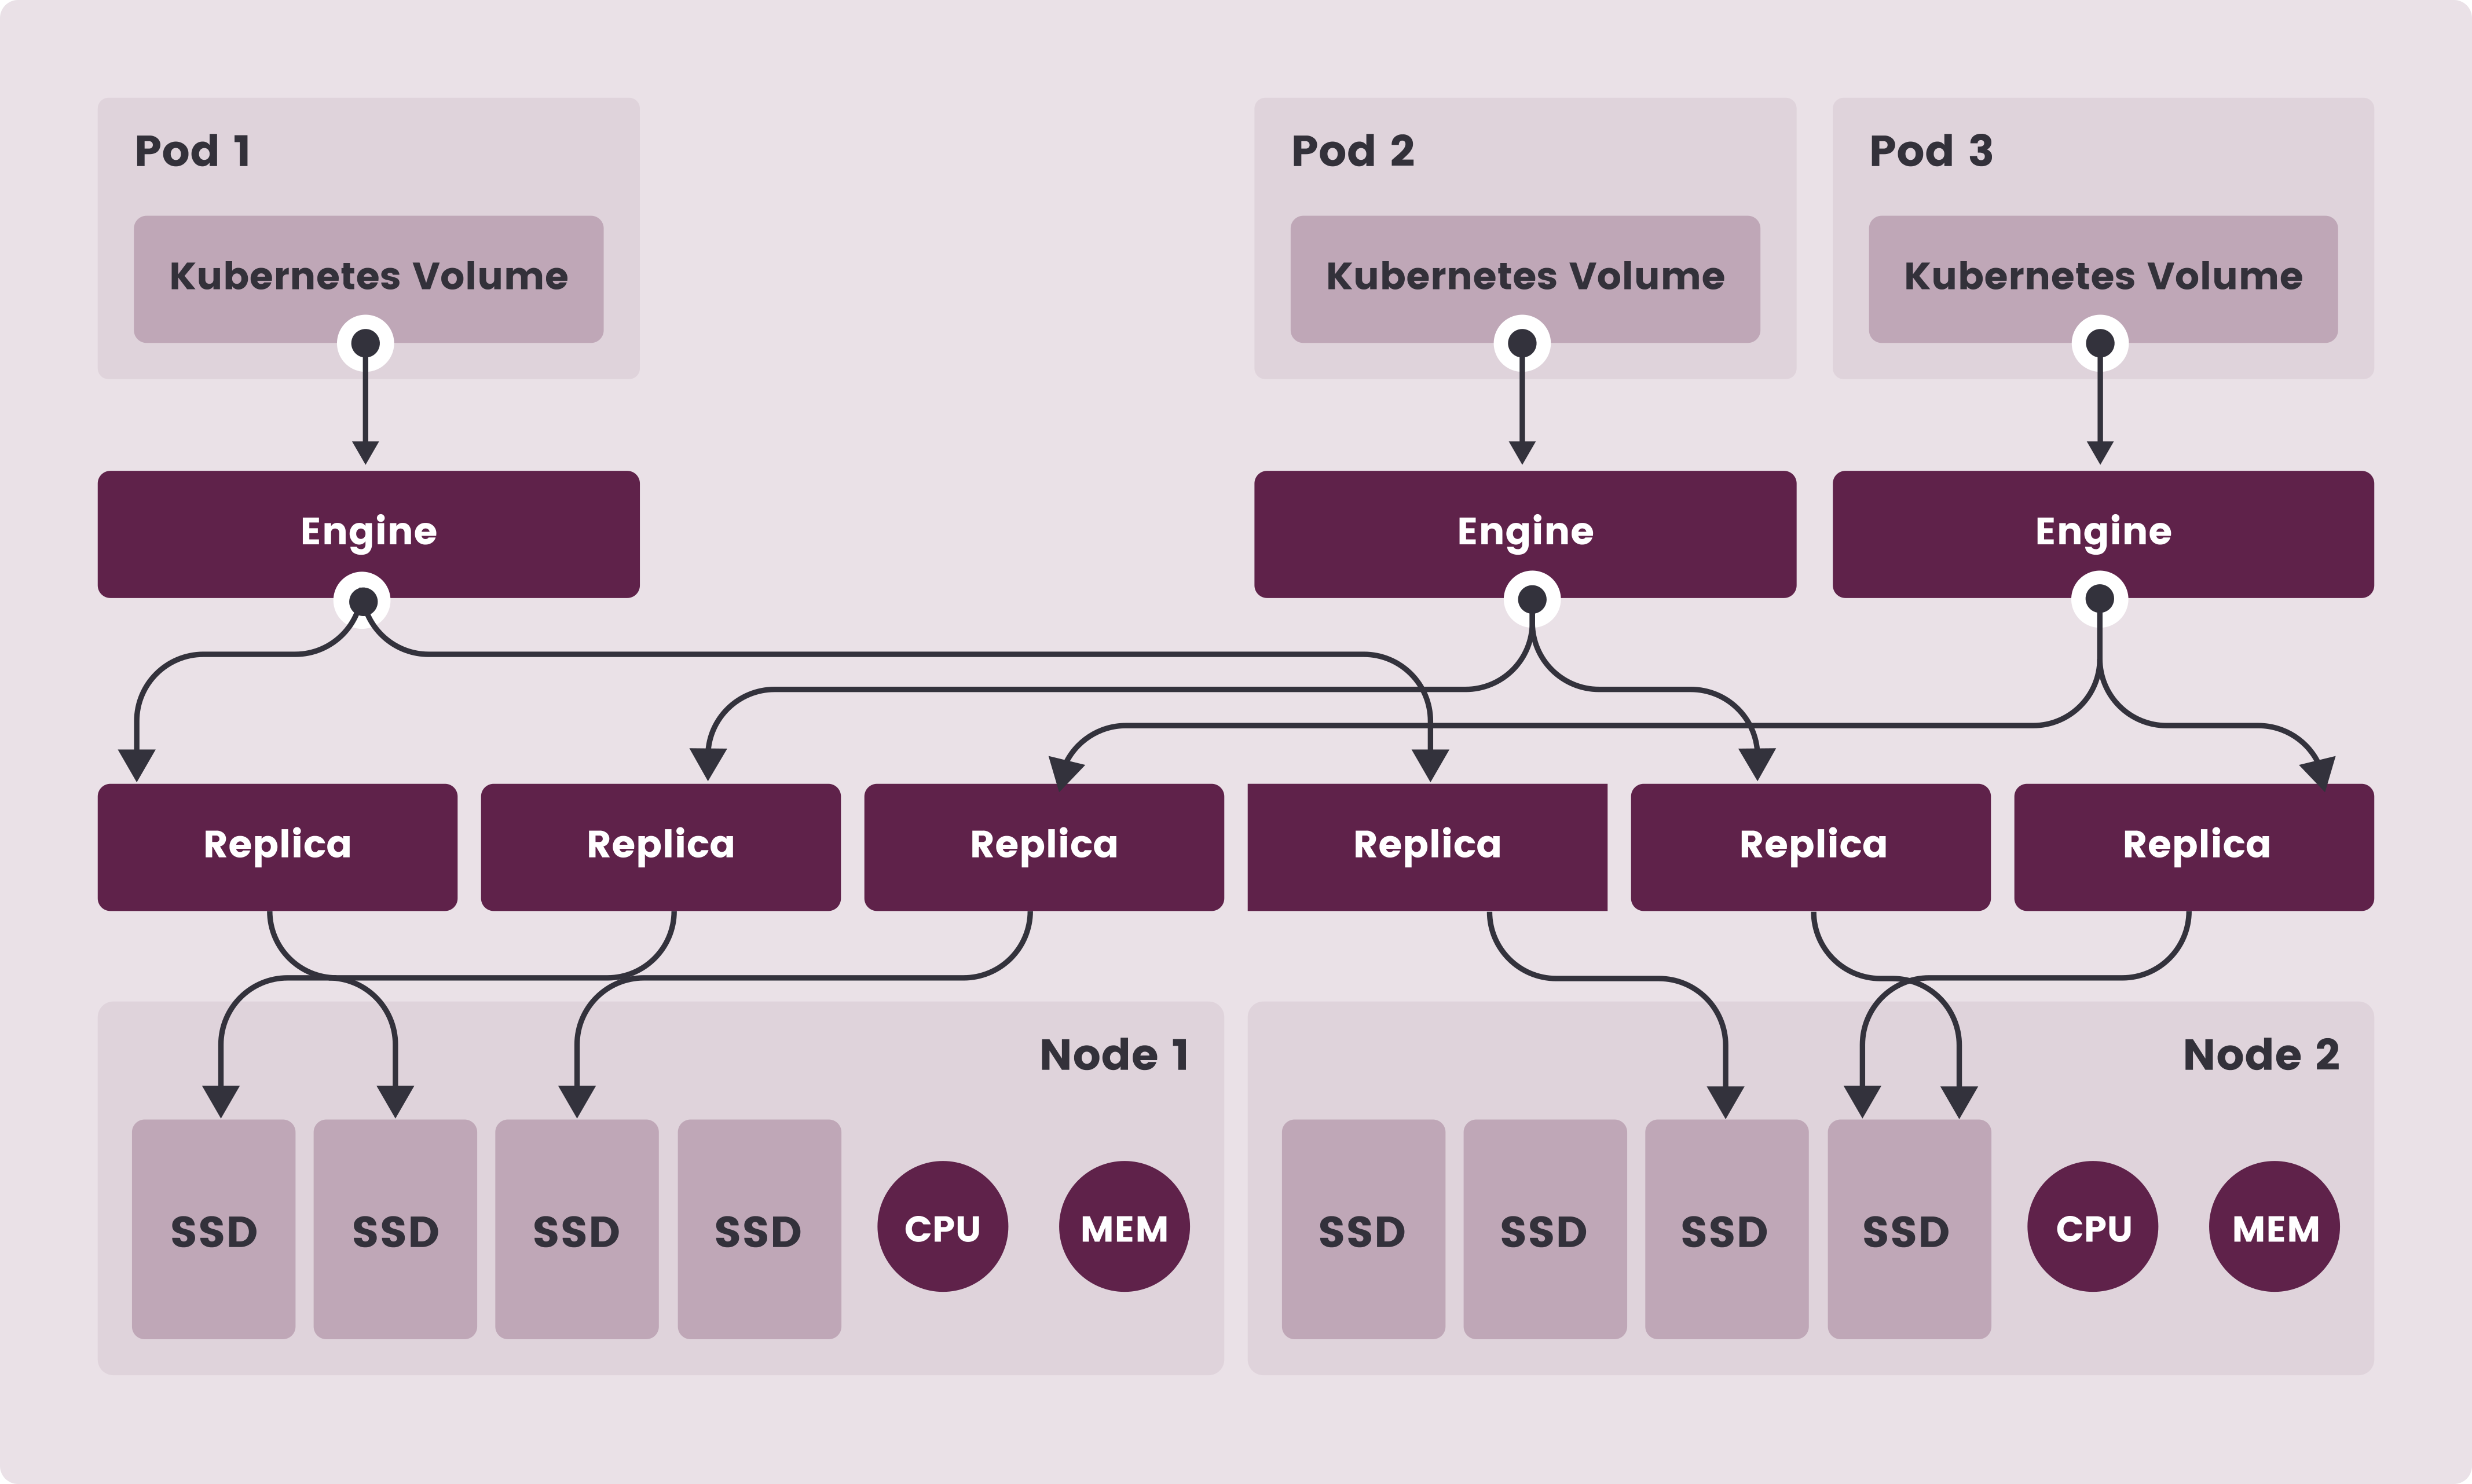
\includegraphics[width=.9\linewidth]{images/recluster/longhorn.png} } %
  {\scriptsize Source: \url{https://longhorn.io} }
  \caption{Longhorn's
  architecture
  overview
  and
  Read/Write
  Data
  Flow
  between
  the
  Volume,
  Longhorn
  Engine,
  Replica
  Instances,
  and
  Disks}
  \label{fig:longhorn}
\end{figure}
It should be mentioned that having an underlying reliable persistent storage for
the whole cluster benefits not just the registry component but also every other Kubernetes
application deployment that requires any type of persistent storage, such as
database and media services.

\subsection{MetalLB}
\label{subsec:implementation_dependencies_metallb}

\begin{wrapfigure}
  {l}{.25\textwidth} %
  \centering
  \def\stackalignment{l}\stackunder{ 
\includegraphics[width=\linewidth]{images/logos/metallb.png} } %
  {\scriptsize \parbox[t]{\linewidth}{ Source: \url{https://metallb.universe.tf}} }
  \caption{MetalLB logo}
\end{wrapfigure}

\subsection{Prometheus}
\label{subsec:implementation_dependencies_prometheus}

\begin{wrapfigure}
  {l}{.25\textwidth} %
  \centering
  \def\stackalignment{l}\stackunder{ 
\includegraphics[width=\linewidth]{images/logos/prometheus.png} } %
  {\scriptsize \parbox[t]{\linewidth}{ Source: \url{https://prometheus.io}} }
  \caption{Prometheus logo}
\end{wrapfigure}

Prometheus is an Open Source system that is specifically designed for monitoring
and alerting. It is the only system that Kubernetes natively supports and the de
facto standard across the Cloud Native ecosystem\cite{prometheus_overview_faq}. Prometheus
joined CNCF in 2016 as the second hosted project with a Graduated maturity level,
only after Kubernetes itself\footnote{\url{https://www.cncf.io/projects/prometheus}}\cite{prometheus_overview}.
Prometheus has no mapping to a cluster component, and the architecture overview indicates
no monitoring component at all. This is because having Prometheus deployed and
continually operating in the cluster is a choice of the organization operating
the cluster rather than a hard necessity; even if the Metrics Server is required
on each Node. Furthermore, Prometheus may be deployed outside of the cluster environment
and configured to access node metrics from the external network, or it can be
run exclusively for certain periods, allowing monitoring of the cluster for testing
or performance evaluation. Nonetheless, Prometheus remains an important tool for
monitoring and analyzing how the cluster is behaving, which is why it is
specified as a dependency and is also included in the final archive bundle.

As previously stated, Prometheus' primary function is to collect metrics data
generated by exporters and query/interpolate this data. Moreover, Prometheus can
monitor itself since, like Node Exporter, it provides its metrics via an HTTP
endpoint. There is a plethora of available exporters and possible integrations\footnote{\url{https://prometheus.io/docs/instrumenting/exporters}}.
In addition to the default exporter installed on each node in the cluster
implementation, an organization managing the cluster can choose to add as many exporters
as the number of components and applications running on it, resulting in a
better, clearer, and finer-grained overview of the entire cluster status both in
real-time and over a period. For example, in addition to the Database component,
it is possible to install its corresponding exporter, which allows the
monitoring of Database metrics such as health, performance and resource usage.

\subsubsection{Features}
\label{subsubsec:implementation_dependencies_prometheus_features}

Prometheus has several features\footnote{\url{https://prometheus.io/docs/introduction/overview/\#features}},
but the two most essential for the cluster implementation are described below\cite{prometheus_overview}:
\begin{enumerate}
  \item A multidimensional data model that contains time series data that is uniquely
    identified by metric name and optional key-value pairs known as labels. Time
    series data are streams of timestamped values from the same metric and set
    of labeled dimensions\cite{prometheus_data_model}.
    \begin{enumerate}
      \item \texttt{Metrics}
        \newline
        The metric name, which is sometimes complemented by a short description (\lstinline[language=prometheus]{# HELP ...}),
        defines the overall system characteristic being monitored.
        \newline
        For example, \lstinline[language=prometheus, alsoletter={_},
        morekeywords={node_memory_MemFree_bytes}]{node_memory_MemFree_bytes}
        metric defines the total amount of physical memory (in bytes) that is
        not in use.
        \newline
        Each metric has a distinct type (\lstinline[language=prometheus]{# TYPE ...}).
        There is a total of four different types of metrics, which are briefly outlined
        below\cite{prometheus_metric_types}:
        \begin{enumerate}
          \item \texttt{Counter}
            \newline
            A cumulative metric that depicts a single monotonically increasing
            counter, the value of which can only increase or be reset to zero\footnote{\url{https://prometheus.io/docs/concepts/metric_types/\#counter}}.

          \item \texttt{Gauge}
            \newline
            A metric that represents a single numerical value that can vary
            arbitrarily up and down\footnote{\url{https://prometheus.io/docs/concepts/metric_types/\#gauge}}.

          \item \texttt{Histogram}
            \newline
            Samples and counts observations in variable buckets, providing also the
            total sum of all observed values\footnote{\url{https://prometheus.io/docs/concepts/metric_types/\#histogram}}.

          \item \texttt{Summary}
            \newline
            Similar to \texttt{Histogram} type, it also calculates configurable
            quantiles over a time window\footnote{\url{https://prometheus.io/docs/concepts/metric_types/\#summary}}.
        \end{enumerate}

      \item \texttt{Labels}
        \newline
        Labels allow Prometheus' dimensional data model: each given combination
        of labels for the same metric name identifies a unique dimensional
        instantiation of that metric. These dimensions can be used to filter and
        aggregate data by the \texttt{PromQL} query language.
        \newline
        For example, \lstinline[language=prometheus, alsoletter={_},
        morekeywords={node_cpu_seconds_total}, morekeywords={[2]{cpu, mode}}]|node_cpu_seconds_total{cpu="0",mode="idle"}|,
        determines the number of seconds spent in idle mode by CPU core 0.
    \end{enumerate}

  \item Prometheus includes a functional and extensible query language known as PromQL\footnote{\url{https://prometheus.io/docs/prometheus/latest/querying/basics}}
    (Prometheus Query Language) that allows the selection and aggregation of time
    series data in real-time. The outcome of an expression can be shown as a
    graph, tabulated data, or consumed by external systems (such as Grafana, see
    section \ref{subsubsec:implementation_dependencies_prometheus_grafana}) via the
    HTTP API\cite{prometheus_promql}.
\end{enumerate}

Two examples of \texttt{PromQL} queries that have been widely used for cluster monitoring
are shown below. Note of how the various metrics and labels are used for
filtering and aggregation.

Listing \ref{lst:promql_1} illustrates an example of a \texttt{PromQL} query to obtain
the overall CPU usage in percent (\texttt{0} to \texttt{100}). Because the
metric \lstinline[language=prometheus, alsoletter={_}, morekeywords={node_cpu_seconds_total}]{node_cpu_seconds_total}
is of type \texttt{counter}, the considered value is limited to the last one
minute (\texttt{1m}).

\begin{lstlisting}[language=promql, numbers=none, alsoletter={_01}, morekeywords={[2]{node_cpu_seconds_total}}, morekeywords={[3]{cpu, mode}}, morekeywords={[4]{100, 1, 1m}}, xleftmargin=\parindent, label={lst:promql_1}, caption=\texttt{PromQL} query to obtain overall CPU usage in percent]
  100 * (avg without (mode, cpu) (1 - rate(node_cpu_seconds_total{mode="idle"}[1m])))
\end{lstlisting}

Listing \ref{lst:promql_2} illustrates an example of a \texttt{PromQL} query to obtain
the amount of memory usage in percent (\texttt{0} to \texttt{100}).

\begin{lstlisting}[language=promql, numbers=none, alsoletter={_, 0, 1}, morekeywords={[2]{node_memory_MemTotal_bytes, node_memory_MemFree_bytes}}, morekeywords={[4]{100}}, xleftmargin=\parindent, label={lst:promql_2}, caption=\texttt{PromQL} query to obtain the amount of memory usage in percent]
  100 * ((node_memory_MemTotal_bytes - node_memory_MemFree_bytes) / node_memory_MemTotal_bytes)
\end{lstlisting}

\subsubsection{Grafana}
\label{subsubsec:implementation_dependencies_prometheus_grafana}

\begin{wrapfigure}
  {l}{.25\textwidth} %
  \centering
  \def\stackalignment{l}\stackunder{ 
\includegraphics[width=\linewidth]{images/logos/grafana.png} } %
  {\scriptsize \parbox[t]{\linewidth}{ Source: \url{https://grafana.com}} }
  \caption{Grafana logo}
\end{wrapfigure}

Prometheus is frequently used in conjunction with Grafana\footnote{\url{https://grafana.com/grafana}},
an interactive data visualization platform\cite{grafana}. \\ %
Prometheus collects metrics and provides the sophisticated \texttt{PromQL} query
language; Grafana then translates these metrics and/or query results into
relevant charts and graphs that may be consolidated into one or more dashboards.
\\ %
It should be noted that Grafana is not considered a dependency in the cluster
implementation and therefore is not distributed in the release archive bundle.

\subsection{Management}
\label{subsec:implementation_dependencies_management}

\subsubsection{Configuration}
\label{subsec:implementation_dependencies_management_configuration}

\begin{lstlisting}[language=yaml, alsoletter={.}, morekeywords={[2]{autoscaler, k3s, node_exporter, prometheus, url, assets, releases, files, LICENSE, install.sh}}, xleftmargin=\parindent, caption=TODO]
  autoscaler:
    url: "https://github.com/carlocorradini/autoscaler"
    assets:
      - "cluster-autoscaler.amd64.tar.gz"
      - "cluster-autoscaler.arm64.tar.gz"
    releases:
      - "latest"
    files:
      LICENSE: "https://raw.githubusercontent.com/carlocorradini/autoscaler/master/LICENSE"

  k3s:
    url: "https://github.com/k3s-io/k3s"
    assets:
      - "k3s"
      - "k3s-arm64"
      - "k3s-airgap-images-amd64.tar.gz"
      - "k3s-airgap-images-arm64.tar.gz"
    releases:
      - "latest"
    files:
      LICENSE: "https://raw.githubusercontent.com/k3s-io/k3s/master/LICENSE"
      install.sh: "https://raw.githubusercontent.com/k3s-io/k3s/master/install.sh"

  node_exporter:
    url: "https://github.com/prometheus/node_exporter"
    assets:
      - "node_exporter-[0-9]+.[0-9]+.[0-9]+.linux-amd64.tar.gz"
      - "node_exporter-[0-9]+.[0-9]+.[0-9]+.linux-arm64.tar.gz"
    releases:
      - "latest"
    files:
      LICENSE: "https://raw.githubusercontent.com/prometheus/node_exporter/master/LICENSE"
      install.sh: "https://raw.githubusercontent.com/carlocorradini/node_exporter_installer/main/install.sh"

  prometheus:
    url: "https://github.com/prometheus/prometheus"
    assets:
      - "prometheus-[0-9]+.[0-9]+.[0-9]+.linux-amd64.tar.gz"
      - "prometheus-[0-9]+.[0-9]+.[0-9]+.linux-arm64.tar.gz"
    releases:
      - "latest"
    files:
      LICENSE: "https://raw.githubusercontent.com/prometheus/prometheus/main/LICENSE"
\end{lstlisting}

\subsubsection{Script}
\label{subsec:implementation_dependencies_management_script}

\begin{xltabular}
  {\textwidth} { >{\ttfamily}l | X | >{\ttfamily}c }

  \multicolumn{1}{ c |}{\large{\textbf{Name}}} &
  \multicolumn{1}{ c |}{\large{\textbf{Description}}} &
  \multicolumn{1}{ c }{\large{\textbf{Default Value}}} \\ \hhline{===}

  --config-file <FILE> & & dependencies.config.yaml \\ \hline

  --help & & \\ \hline

  --log-level <LEVEL> & & info \\ \hline

  --sync & & \\ \hline

  --sync-force & & \\ \hline
\end{xltabular}

\section{Installer}
\label{sec:implementation_installer}

\subsection{POSIX Shell}
\label{subsec:implementation_installer_posix_shell}

\subsection{Configuration Arguments}
\label{subsec:implementation_installer_configuration_arguments}

\subsection{Configuration Files}
\label{subsec:implementation_installer_configuration_files}

\subsubsection{Certificates}
\label{subsubsec:implementation_installer_configuration_files_certificates}

\subsubsection{K3s}
\label{subsubsec:implementation_installer_configuration_files_k3s}

\subsubsection{K8s}
\label{subsubsec:implementation_installer_configuration_filesn_k8s}

\subsubsection{Node exporter}
\label{subsubsec:implementation_installer_configuration_files_node_exporter}

\subsubsection{reCluster}
\label{subsubsec:implementation_installer_configuration_files_recluster}

\subsubsection{SSH}
\label{subsubsec:implementation_installer_configuration_files_ssh}

\subsection{Node Facts}
\label{subsec:implementation_installer_node_facts}

\subsection{Node Information}
\label{subsec:implementation_installer_node_information}

\subsection{Node Benchmarks}
\label{subsec:implementation_installer_node_benchmarks}

\subsubsection{SysBench}
\label{subsubsec:implementation_installer_node_benchmarks_sysbench}

\subsection{Node Power Consumption}
\label{subsec:implementation_installer_node_power_consumption}

\subsubsection{CloudFree Smart Plug}
\label{subsubsec:implementation_installer_node_power_consumption_cloudfree_smart_plug}

\subsection{Node Registration}
\label{subsec:implementation_installer_node_registration}

\subsubsection{K8s Node Label And Name}
\label{subsubsec:implementation_installer_node_registration_k8s_node_label_and_name}

\subsection{Cluster Initialization}
\label{subsec:implementation_installer_cluster_initialization}

\subsubsection{Kubeconfig}
\label{subsubsec:implementation_installer_cluster_initialization_kubeconfig}

\subsubsection{Database}
\label{subsubsec:implementation_installer_cluster_initialization_database}

\subsubsection{Server}
\label{subsubsec:implementation_installer_cluster_initialization_server}

\subsubsection{Admin And Autoscaler Users}
\label{subsubsec:implementation_installer_cluster_initialization_admin_and_autoscaler_users}

\subsubsection{K8s}
\label{subsubsec:implementation_installer_cluster_initialization_k8s}

\subsection{Services}
\label{subsec:implementation_installer_services}

\subsubsection{Start}
\label{subsubsec:implementation_installer_services_start}

\subsubsection{Stop}
\label{subsubsec:implementation_installer_services_stop}

\subsubsection{Boot}
\label{subsubsec:implementation_installer_services_boot}

\subsubsection{Shutdown}
\label{subsubsec:implementation_installer_services_shutdown}

\section{Server}
\label{sec:implementation_server}

\subsection{Database}
\label{subsec:implementation_server_database}

\subsubsection{PostgreSQL}
\label{subsubsec:implementation_server_database_postgresql}

\begin{wrapfigure}
  {r}{.25\textwidth} %
  \centering
  \def\stackalignment{r}\stackunder{ 
\includegraphics[width=\linewidth]{images/logos/postgresql.png} } %
  {\scriptsize \parbox[t]{\linewidth}{ Source: \url{https://wiki.postgresql.org/wiki/Logo}} }
  \caption{PostgreSQL logo}
\end{wrapfigure}

\subsubsection{Prisma}
\label{subsubsec:implementation_server_database_prisma}

\begin{wrapfigure}
  {r}{.25\textwidth} %
  \centering
  \def\stackalignment{r}\stackunder{ 
\includegraphics[width=\linewidth]{images/logos/prisma.png} } %
  {\scriptsize \parbox[t]{\linewidth}{ Source: \url{https://www.prisma.io}} }
  \caption{Prisma logo}
\end{wrapfigure}

\subsubsection{Schema}
\label{subsubsec:implementation_server_database_schema}

\subsection{GraphQL}
\label{subsec:implementation_server_graphql}

\subsubsection{GraphQL vs REST}
\label{subsubsec:implementation_server_graphql_graphql_vs_rest}

\subsubsection{Schema}
\label{subsubsec:implementation_server_graphql_schema}

\subsection{Node Pool}
\label{subsec:implementation_server_node_pool}

\subsection{Node Registration}
\label{subsec:implementation_server_node_registration}

\subsubsection{JSON Web Token}
\label{subsubsec:implementation_server_node_registration_json_web_token}

\subsection{Upscaling}
\label{subsec:implementation_server_upscaling}

\subsubsection{Wake-on-LAN}
\label{subsubsec:implementation_server_scale_up_wake_on_lan}

\subsection{Downscaling}
\label{subsec:implementation_server_downscaling}

\subsubsection{SSH}
\label{subsubsec:implementation_server_scale_up_ssh}

\section{Autoscaling}
\label{sec:implementation_autoscaling}

\subsection{Autoscaler}
\label{subsec:implementation_autoscaling_autoscaler}

\subsection{Vertical Pod Autoscaler}
\label{subsec:implementation_autoscaling_vertical_pod_autoscaler}

\subsection{Horizontal Pod Autoscaler}
\label{subsec:implementation_autoscaling_horizontal_pod_autoscaler}

\subsection{Cluster Autoscaler}
\label{subsec:implementation_autoscaling_cluster_autoscaler}

\subsubsection{Cloud Provider}
\label{subsubsec:implementation_autoscaling_cluster_autoscaler_cloud_provider}

\subsubsection{Configuration}
\label{subsubsec:implementation_autoscaling_cluster_autoscaler_configuration}

% TODO Cloud Configuration

\subsubsection{Upscaling}
\label{subsubsec:implementation_autoscaling_cluster_autoscaler_upscaling}

\subsubsection{Downscaling}
\label{subsubsec:implementation_autoscaling_cluster_autoscaler_downscaling}